\chapter{System Architecture and Detailed Design}
\label{ch:architecture}

This chapter presents a comprehensive exposition of the software architecture, microservice decomposition principles, identity security boundaries, and real-time geospatial coordination mechanisms underpinning the VietForecast platform. The architecture is engineered to satisfy three paramount design objectives: independent scalability across heterogeneous workload profiles, uncompromising integrity and freshness of surface meteorological observations for traffic safety, and rigorous isolation of backend system secrets and user session state against modern web application attack vectors.

\section{System Architecture Overview and C4 Container Model}
\label{sec:arch_overview_c4}

\subsection{Microservice Architecture and Component Decomposition}
To reconcile the profound disparity in execution lifecycles and workload dynamics between interactive client-facing operations (map navigation, rapid point lookups, conversational queries) and prolonged asynchronous background pipelines (periodic 63-province data polling, schema normalization, spatial indexing), VietForecast adopts a distributed microservices topology encapsulated within containerized environments.

Figure~\ref{fig:c4_container_en} depicts the C4 Model Level 2 (Container Diagram) of the VietForecast platform, delineating network boundaries, containerized execution units, and communication protocols over standardized interfaces.

\begin{figure}[H]
\centering
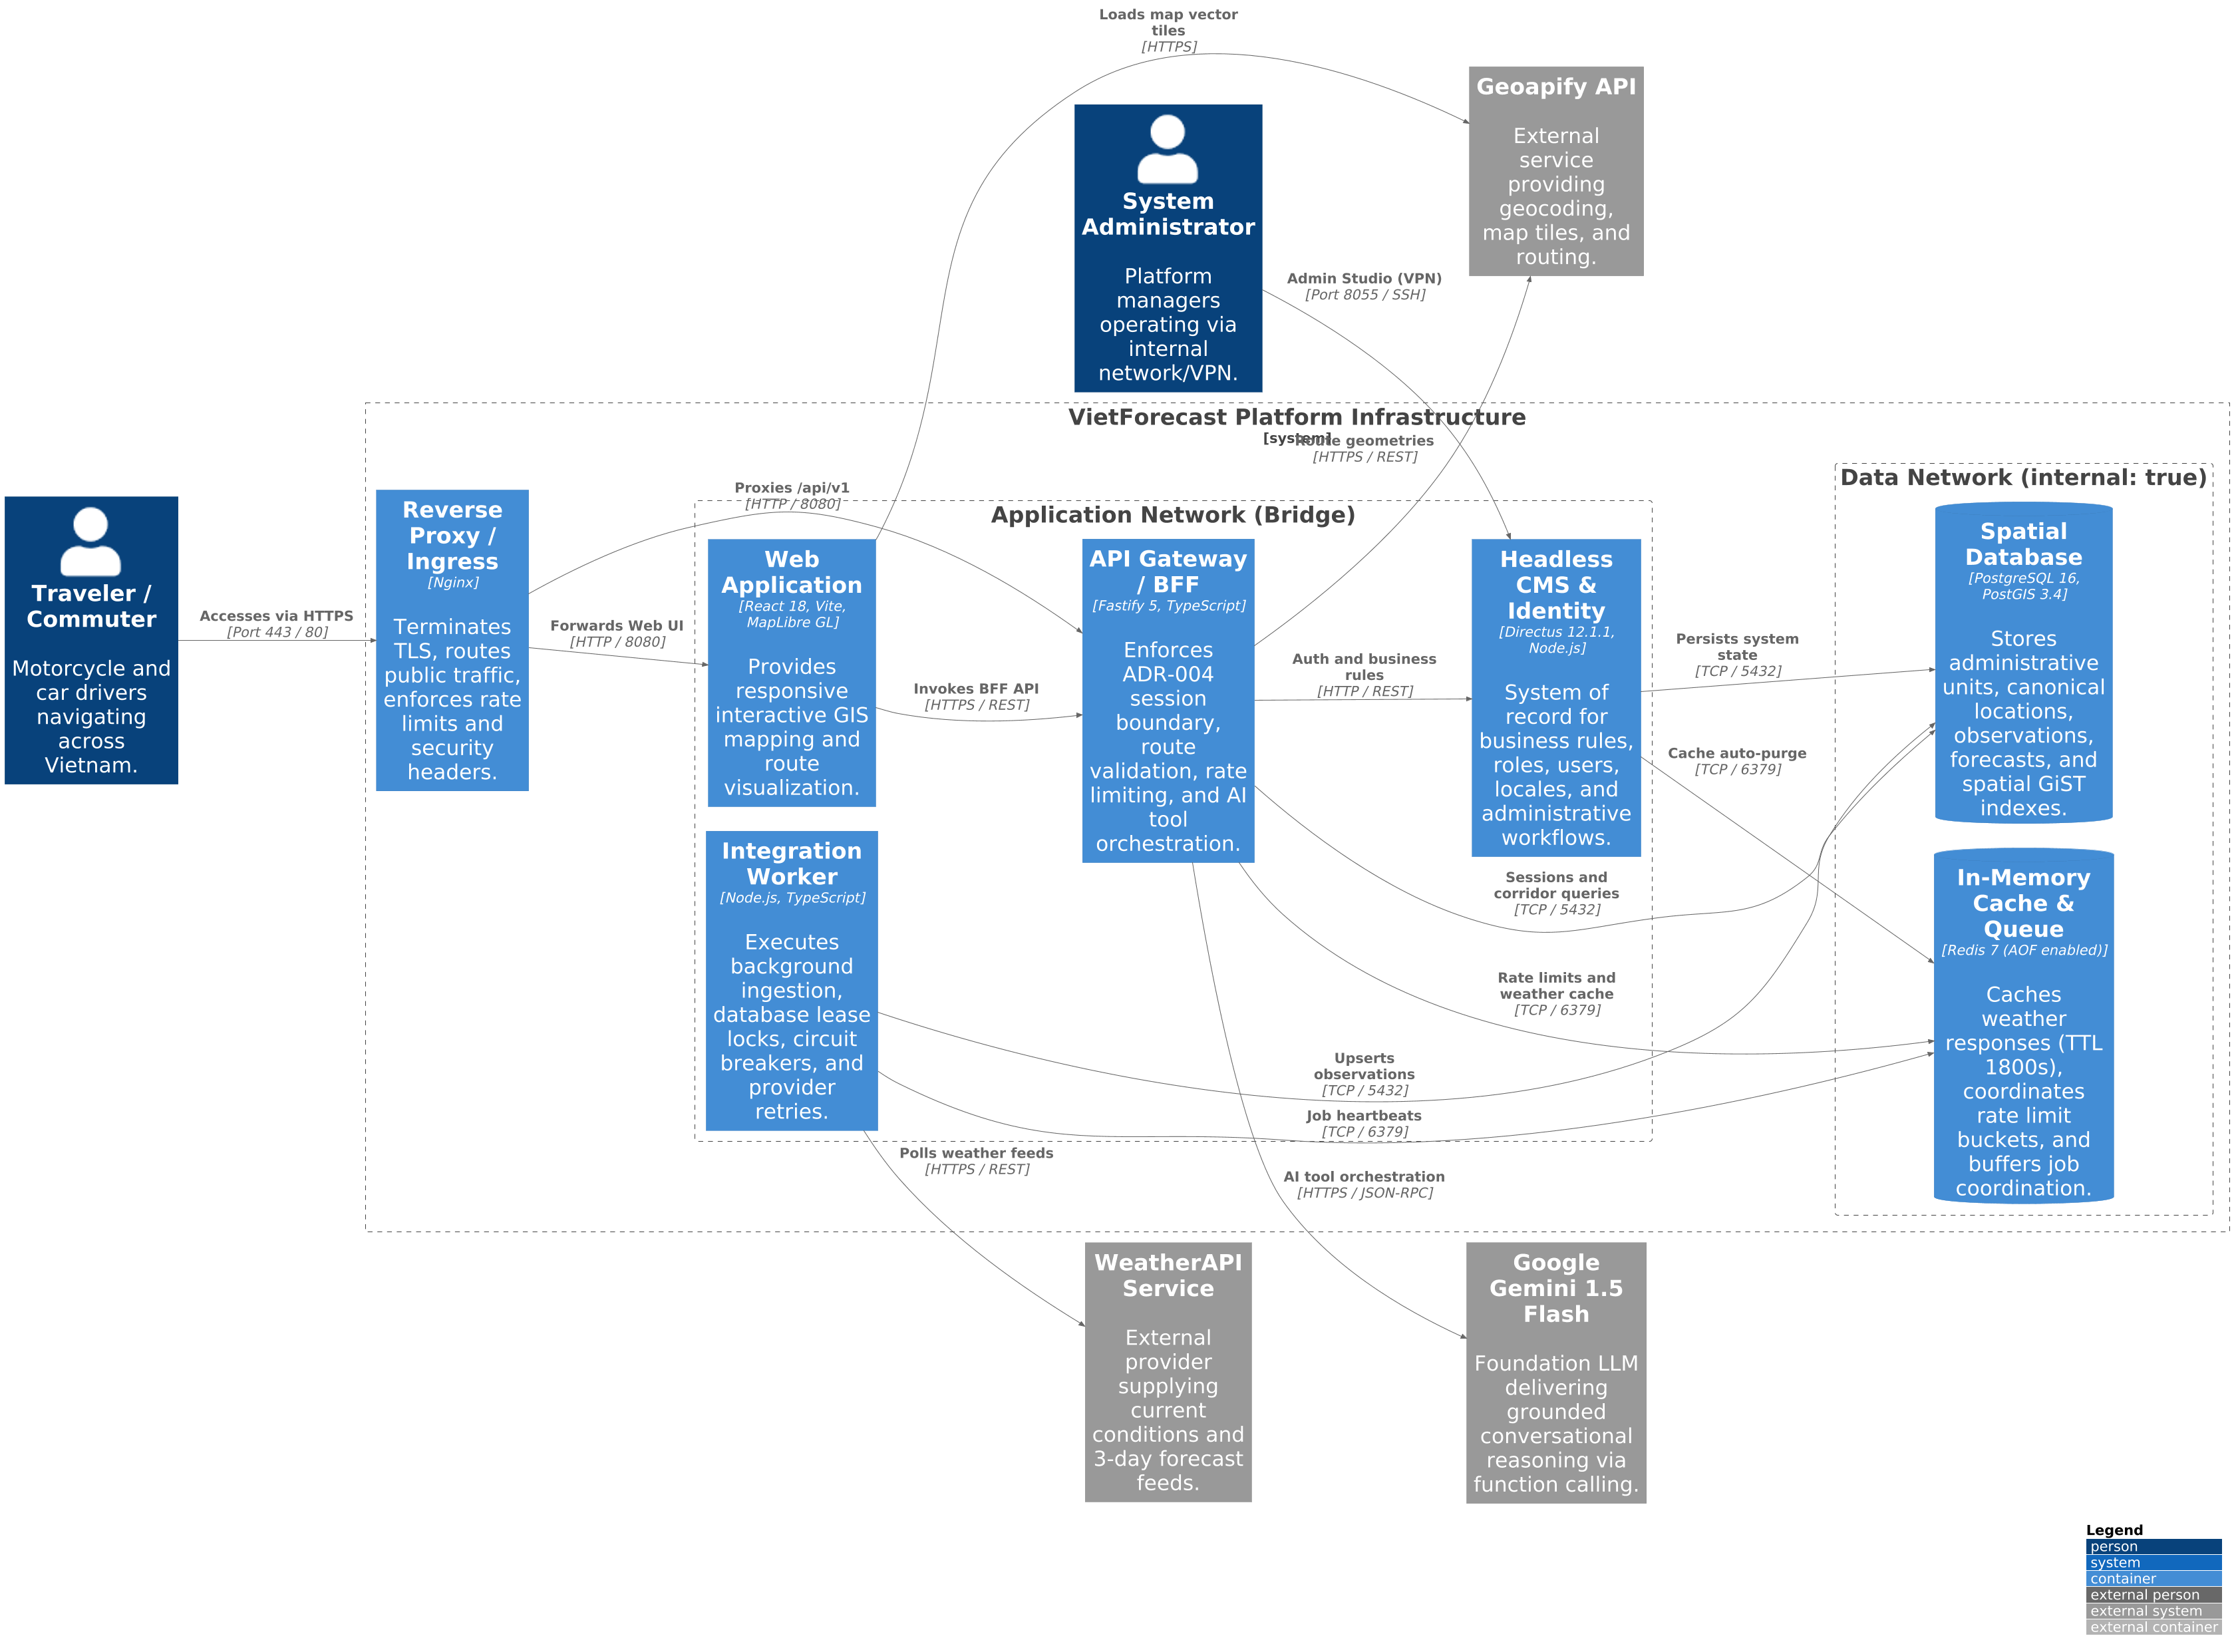
\includegraphics[width=0.95\textwidth, height=0.65\textheight, keepaspectratio]{figures/c4_container.png}
\caption[C4 Container Diagram (Level 2) of VietForecast]{C4 Container Diagram (Level 2) illustrating the microservice topology and network segmentation of the VietForecast platform.}
\label{fig:c4_container_en}
\end{figure}

Technical responsibilities across system containers are strictly partitioned under the principle of separation of concerns:
\begin{itemize}
    \item[-] Reverse proxy and TLS termination (\textit{Nginx Reverse Proxy}): Operates as the sole public ingress point from the external Internet on standard ports 80 and 443. This component terminates TLS/HTTPS sessions, injects strict HTTP security headers (Content Security Policy, Strict-Transport-Security, X-Frame-Options), routes incoming traffic to either the web presentation layer or the API gateway, and enforces network-level rate limiting to safeguard downstream microservices.
    \item[-] Web user interface application (\textit{Web Application}): Implemented as a responsive Single Page Application utilizing React 18, Vite build tooling, and the MapLibre GL 4 spatial rendering engine. The application provides dynamic geospatial interaction at 60 frames per second through WebGL hardware acceleration, visualizes multi-layer raster weather overlays, and renders three-dimensional route trajectories. Crucially, the web application maintains zero provider credentials or direct database connections.
    \item[-] Service gateway and backend-for-frontend (\textit{Fastify API / BFF}): Engineered with Fastify 5 and TypeScript to serve as the unified Backend-For-Frontend (BFF). This container terminates browser-initiated requests, enforces session integrity, applies endpoint rate limiting via Redis token buckets, coordinates multi-objective route hazard scoring, and acts as the secure execution mediator for grounded function calling with Google Gemini 1.5 Flash.
    \item[-] Headless content management and identity authority (\textit{Directus 12.1.1}): Functions as the authoritative System of Record for user accounts, role-based access control (RBAC), administrative hierarchies across Vietnam's 63 provinces, risk rule thresholds, and localized strings. The Directus version is explicitly pinned to release 12.1.1 to guarantee absolute schema stability and administrative studio consistency.
    \item[-] Background integration worker (\textit{Integration Worker}): A decoupled Node.js service dedicated to executing latency-intensive, scheduled, and network-bound workflows. Key responsibilities include polling observation feeds from WeatherAPI across all provinces, normalizing metrics into WMO-compliant representations, computing SHA-256 integrity checksums, and orchestrating database lease acquisitions.
    \item[-] Relational spatial database (\textit{PostgreSQL 16 + PostGIS 3.4}): Constitutes the persistent data store of the platform, offering native support for Open Geospatial Consortium (OGC) geometry types and geodetic ellipsoidal calculations. Generalized Search Tree (GiST) spatial indexes are established across all coordinate and boundary columns to ensure spatial corridor queries resolve within 50 milliseconds.
    \item[-] In-memory cache and coordination layer (\textit{Redis 7}): Configured with Append-Only File (AOF) durability to provide ultra-low latency caching for current weather observations (time-to-live TTL of 1,800 seconds), coordinate rate-limiting token buckets, and buffer inter-service synchronization signals.
\end{itemize}

\subsection{Network Segmentation and Zero-Trust Isolation Policies (Docker Segmentation)}
To thwart lateral movement in the event of an individual container compromise, the Docker infrastructure establishes strict network segmentation through two mutually isolated networks:
\begin{itemize}
    \item[-] Application network (\texttt{application} bridge network): Facilitates inter-service business communication between Nginx, the Web frontend, Fastify API, Directus, and the Integration Worker. Services inside this segment communicate via internal HTTP/REST calls resolved dynamically by Docker DNS.
    \item[-] Data network (\texttt{data} network with \texttt{internal: true}): Represents the highest-security perimeter within the platform. The \texttt{internal: true} flag completely eliminates default gateway routing to the host's external network interfaces. PostgreSQL (port 5432) and Redis (port 6379) bind exclusively to this internal network, rendering them entirely invisible to the public Internet. Any port scanning or credential brute-forcing directed against the database layer is neutralized at the network routing tier.
\end{itemize}

Furthermore, the Directus Admin Studio (listening on port 8055) is strictly bound to the loopback interface (\texttt{127.0.0.1:8055}) pursuant to architectural guidelines ADR-002 and OPS-010. Administrative personnel must establish an authenticated SSH tunnel or connect through an internal Virtual Private Network (VPN) to access administrative capabilities, thereby eliminating exposure to automated public brute-force attacks or zero-day administrative vulnerabilities.

\section{Secure Session Boundary and Identity Architecture (ADR-004)}
\label{sec:auth_session_boundary}

\subsection{Token Exfiltration Vulnerability Analysis and BFF Boundary Architecture}
\label{subsec:token_threat_analysis_en}
In traditional Single Page Application (SPA) architectures, authentication credentials such as JSON Web Tokens (Access Tokens and Refresh Tokens) \cite{rfc7519} are commonly stored within browser client-side storage mechanisms (\texttt{localStorage} or \texttt{sessionStorage}). This convention introduces a catastrophic security vulnerability: any Cross-Site Scripting (XSS) compromise introduced via third-party runtime dependencies grants adversaries direct extraction capability over raw JWTs, facilitating undetectable account impersonation. Furthermore, permitting client browsers to interact directly with upstream Directus instances leaks internal collection schemas and creates an unmaintainable architectural coupling between frontend code and backend database schemas.

To decisively resolve this threat vector, the VietForecast platform adopts the ADR-004 architectural specification, establishing a hardened Backend-For-Frontend (BFF) boundary via the Fastify API. Fastify operates as the sole authenticated gateway: all communication with the Directus identity engine is confined to a private network perimeter, while client browsers never receive, store, or transmit raw JSON Web Tokens.

\subsection{AES-256-GCM Authenticated Encryption Envelope and Opaque Session Handles}
\label{subsec:crypto_envelope_en}
The platform enforces strict Token Isolation and Defense-in-Depth through a multi-tier cryptographic session model:
\begin{itemize}
    \item[-] \textit{Opaque Session Handle}: The Fastify server generates a 32-byte ($256\text{ bits}$) cryptographically secure pseudorandom string utilizing a CSPRNG (\texttt{createOpaque}\allowbreak\texttt{Token(32)}). This handle is dispatched to the client browser exclusively within a hardened cookie named \texttt{\_\_Host-\allowbreak vnwa\_\allowbreak session}, enforcing four foundational security directives: \texttt{HttpOnly} (prohibits JavaScript access via \texttt{document.}\allowbreak\texttt{cookie}), \texttt{Secure} (restricts transmission strictly over encrypted TLS/HTTPS), \texttt{SameSite=Strict} (prevents CSRF in cross-origin requests), and prefix \texttt{\_\_Host-} (binds the cookie immutably to the origin domain).
    \item[-] \textit{One-Way Token Hashing Pattern}: To safeguard active sessions in the event of an unauthorized database dump, the server never persists opaque handles in plaintext. Instead, the handle is passed through a SHA-256 cryptographic hash function before database insertion:
    \begin{equation}
    \label{eq:session_hash_en}
    H_{\text{session}} = \text{SHA-256}(\text{handle})
    \end{equation}
    The resulting 64-character hexadecimal digest $H_{\text{session}}$ serves as the primary key (\texttt{session\_}\allowbreak\texttt{id\_}\allowbreak\texttt{hash}) in \texttt{app\_security.}\allowbreak\texttt{sessions}. Even with full database access, an adversary cannot invert the hash to deduce valid client cookies.
    \item[-] \textit{AES-256-GCM Authenticated Encryption Envelope}: Upstream Directus tokens are encrypted at the Fastify tier employing Advanced Encryption Standard in Galois/Counter Mode (AES-256-GCM) with a 256-bit symmetric server key $K_{\text{enc}} \in \{0, 1\}^{256}$:
    \begin{equation}
    \label{eq:aes_gcm_en}
    \mathcal{C} = \text{AES-GCM-Enc}_{K_{\text{enc}}}(P, \text{IV}), \quad \text{Tag} = \text{GCM-Mac}_{K_{\text{enc}}}(\mathcal{C}, \text{IV})
    \end{equation}
    Every session creation and rotation event generates an independent, random 12-byte initialization vector $\text{IV} \in \{0, 1\}^{96}$ and yields a 16-byte authentication tag $\text{Tag} \in \{0, 1\}^{128}$. The serialization envelope follows the standard structure:
    \begin{equation}
    \label{eq:envelope_format_en}
    \text{Envelope} = \texttt{v1} \,\|\, \text{base64url}(\text{IV}) \,\|\, \text{base64url}(\text{Tag}) \,\|\, \text{base64url}(\mathcal{C})
    \end{equation}
    Encrypted payloads and authentication tags are persisted within the dedicated PostgreSQL table \texttt{app\_security.}\allowbreak\texttt{sessions}. Table permissions are restricted exclusively to the Fastify service role (\texttt{API\_}\allowbreak\texttt{DB\_}\allowbreak\texttt{USER}), precluding even background worker processes from inspecting session states.
\end{itemize}

\subsection{Unified Session Lifecycle: Issuance, Sliding Rotation, and Synchronized Revocation}
\label{subsec:auth_lifecycle_en}
The secure session lifecycle operates through three tightly synchronized stages: initial credential verification and issuance, silent sliding rotation during user activity, and synchronized revocation upon termination or anomalous activity.

\subsubsection{Phase 1: User Authentication and Opaque Session Handle Issuance}
Figure~\ref{fig:seq_auth_lifecycle_p1_en} delineates the sequence execution of user authentication, RBAC authorization assertion, concurrency boundary locking, server-side encryption, and secure cookie issuance.

\begin{figure}[H]
\centering
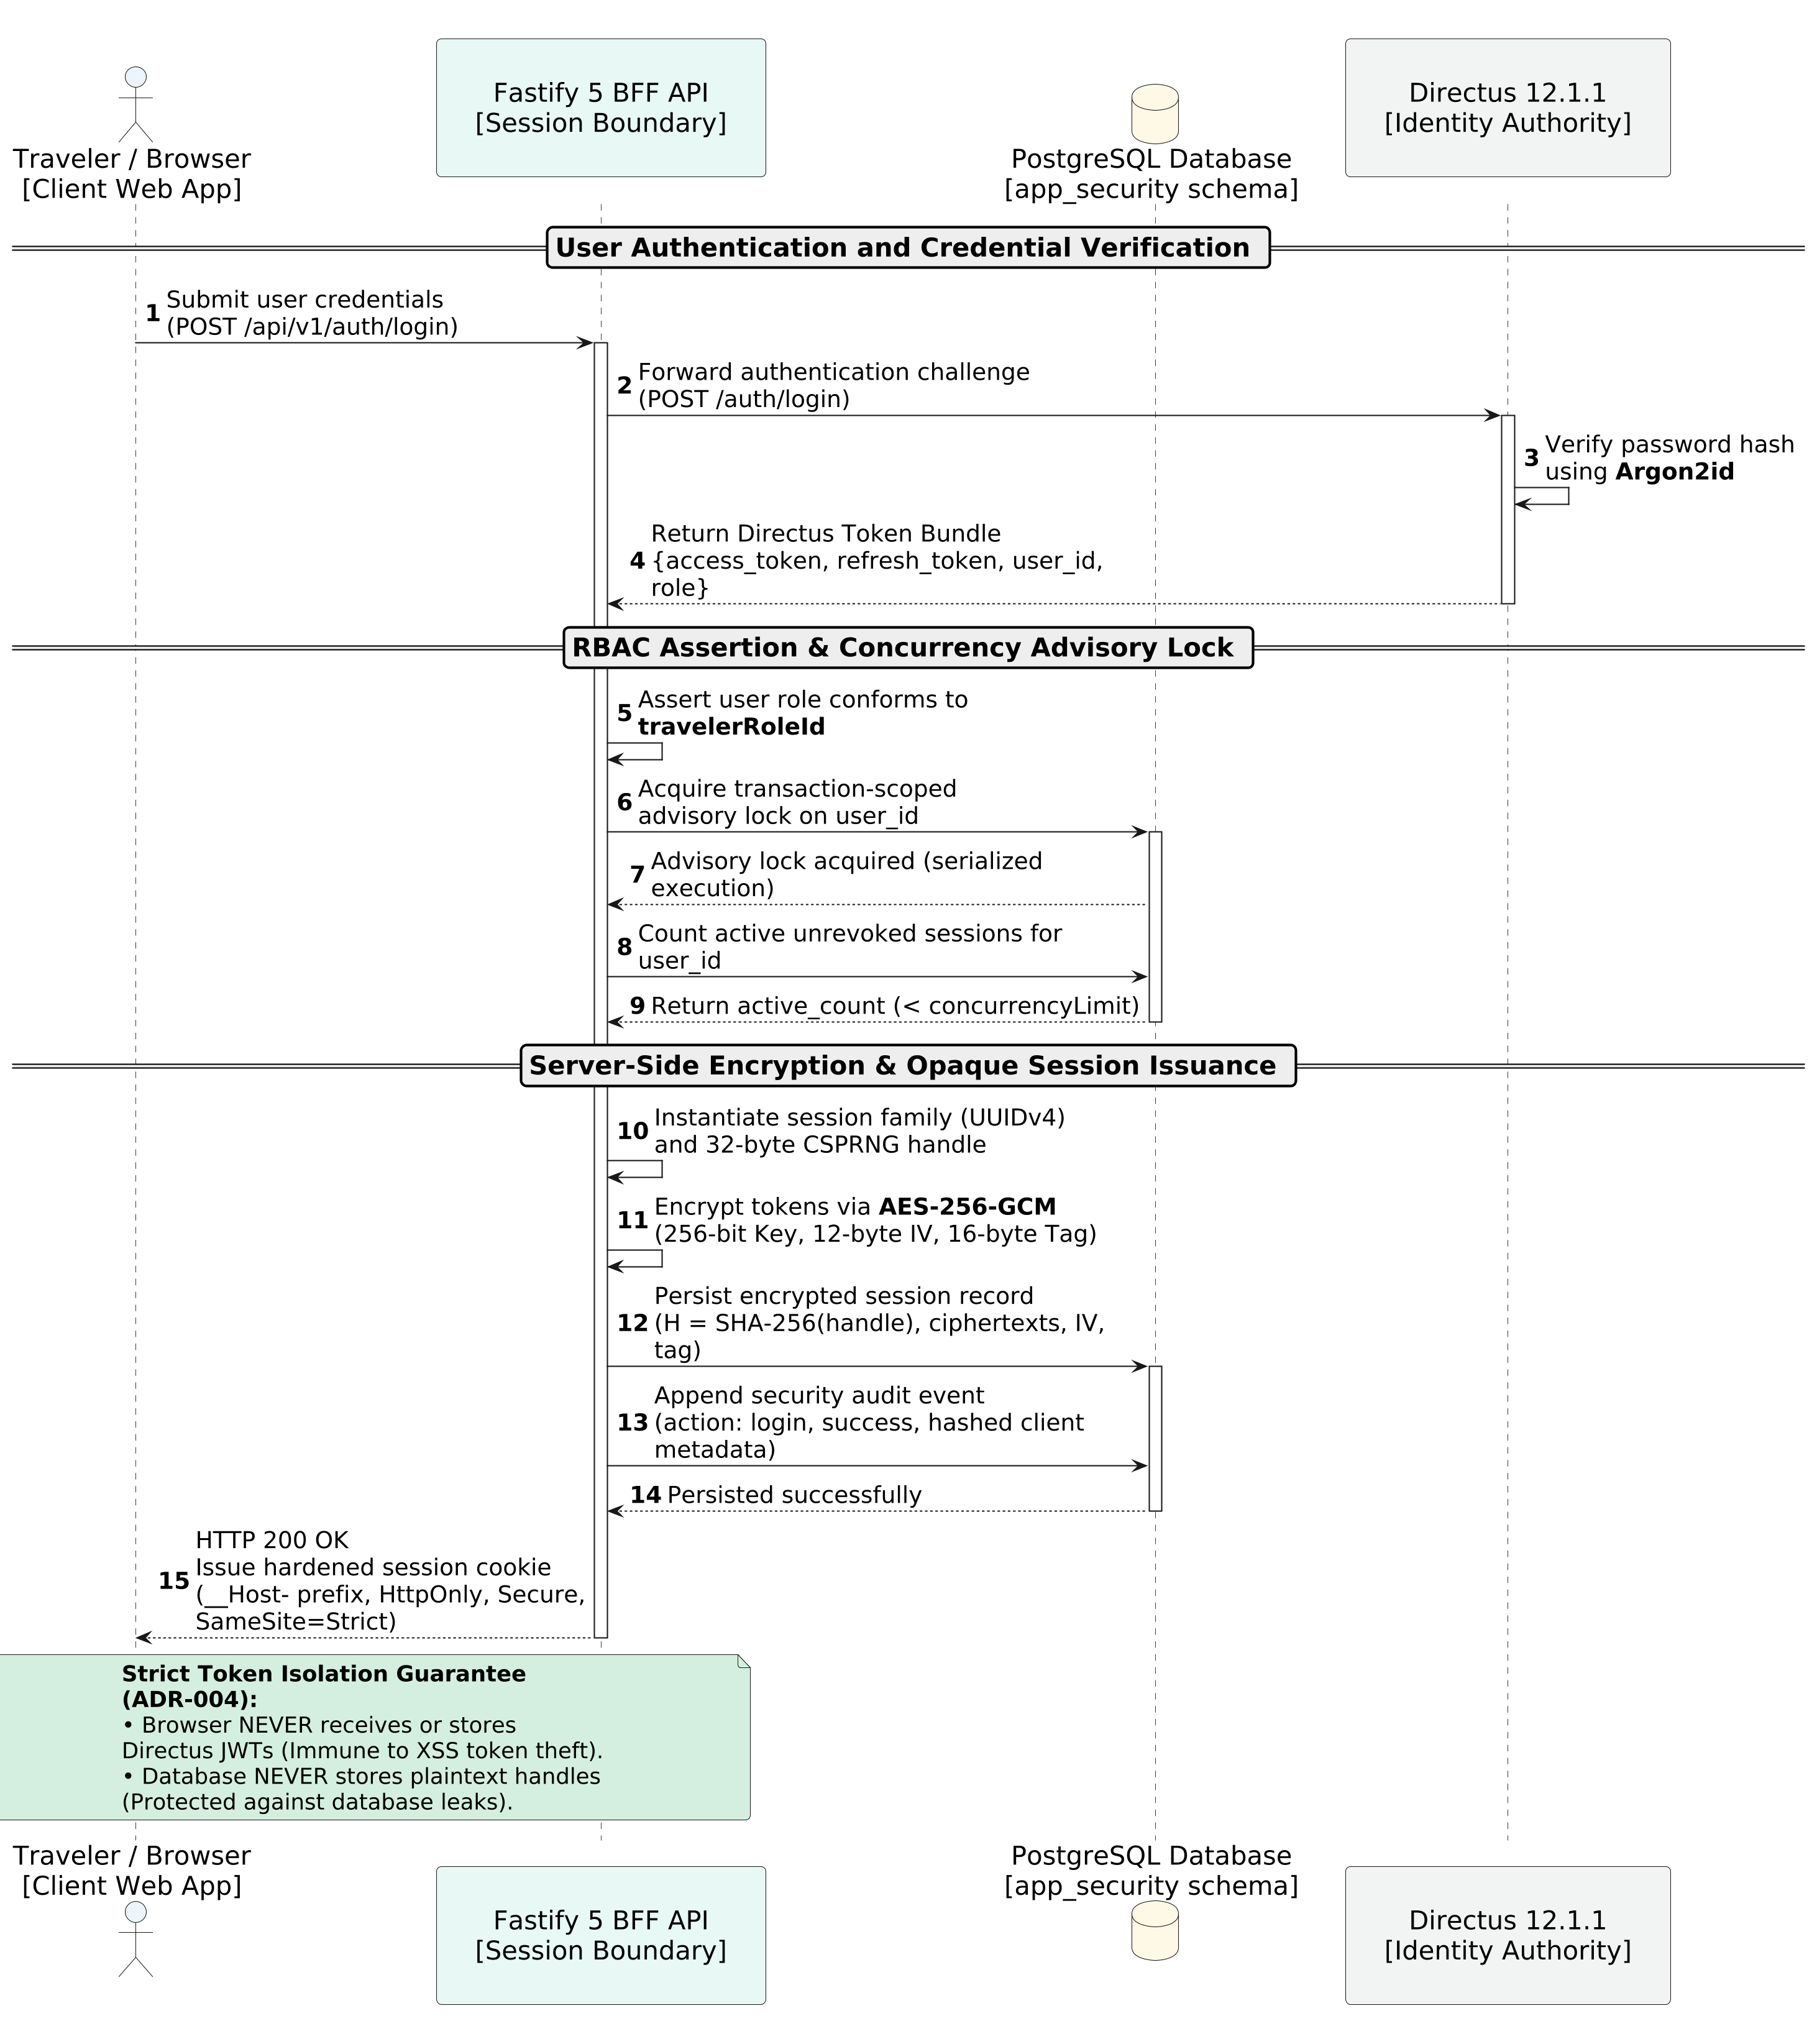
\includegraphics[width=0.92\textwidth, keepaspectratio]{figures/seq_auth_login.png}
\caption[Sequence diagram of session lifecycle (ADR-004) - Phase 1: Session Issuance]{Sequence diagram of the secure session lifecycle (ADR-004) -- Phase 1: User credential authentication, RBAC role assertion, concurrent session bounding, and opaque handle issuance.}
\label{fig:seq_auth_lifecycle_p1_en}
\end{figure}

The operational flow of Phase 1 executes across the following standardized steps:
\begin{itemize}
    \item[-] \textit{Step 1 (Credential dispatch)}: The user submits login credentials (email and password) via the single page application. The client browser transmits a \texttt{POST /api/v1/auth/login} request to the Fastify BFF API gateway. Fastify enforces a Leaky Bucket rate limiter (5 req/min) to thwart automated credential brute-forcing.
    \item[-] \textit{Step 2 (Identity delegation and Argon2id verification)}: Fastify forwards the challenge internally across the \texttt{application} network to Directus Identity Authority. Directus evaluates submitted passwords against stored Argon2id hashes. Upon validation, Directus returns the Directus Token Bundle comprising a short-lived Access Token, a long-lived Refresh Token, the user UUID, and role claims.
    \item[-] \textit{Step 3 (RBAC assertion and concurrent session bounding)}: Fastify verifies that the assigned role corresponds to \texttt{travelerRoleId}. To prevent session proliferation and enforce concurrency boundaries, Fastify acquires a transaction-scoped PostgreSQL advisory lock keyed to $h_u = \text{Hash}_{64}(u)$ and asserts the active session ceiling:
    \begin{equation}
    \label{eq:concurrency_bound_en}
    N_{\text{active}}(u) = \Big| \big\{ s \in \mathcal{S} \;\big|\; s.\text{user\_id} = u \;\wedge\; s.\text{revoked\_at} = \emptyset \big\} \Big| < C_{\text{limit}}
    \end{equation}
    If active sessions reach $C_{\text{limit}}$, the oldest unrevoked session is automatically invalidated to free capacity.
    \item[-] \textit{Step 4 (AES-256-GCM encryption and CSPRNG handle generation)}: Fastify generates a new session family UUIDv4 and a 32-byte cryptographically secure random opaque handle ($h$) using CSPRNG. Upstream Directus JWTs are encrypted with AES-256-GCM using the 256-bit symmetric server key $K_{\text{enc}}$, generating a 12-byte IV and 16-byte authentication Tag.
    \item[-] \textit{Step 5 (One-way token hashing and immutable audit logging)}: Fastify computes digest $H_{\text{session}} = \text{SHA-256}(h)$ and inserts the session record into \texttt{app\_security.sessions}. Simultaneously, an immutable audit event is appended to \texttt{app\_security.audit\_events} capturing login success and privacy-preserving client hashes.
    \item[-] \textit{Step 6 (Hardened cookie dispatch)}: Fastify returns HTTP 200 OK and attaches the hardened \texttt{\_\_Host-vnwa\_session} cookie configured with \texttt{HttpOnly} (mitigating XSS token theft), \texttt{Secure} (mandating TLS transmission), \texttt{SameSite=Strict} (precluding CSRF vectors), and prefix \texttt{\_\_Host-} (enforcing strict domain binding).
\end{itemize}

\subsubsection{Phase 2: Authorized Request Dispatch and Silent Sliding Rotation}
Figure~\ref{fig:seq_auth_lifecycle_p2_en} details the sequence flow for handling authorized business queries, verifying session digests, and executing transparent sliding rotation.

\begin{figure}[H]
\ContinuedFloat
\centering
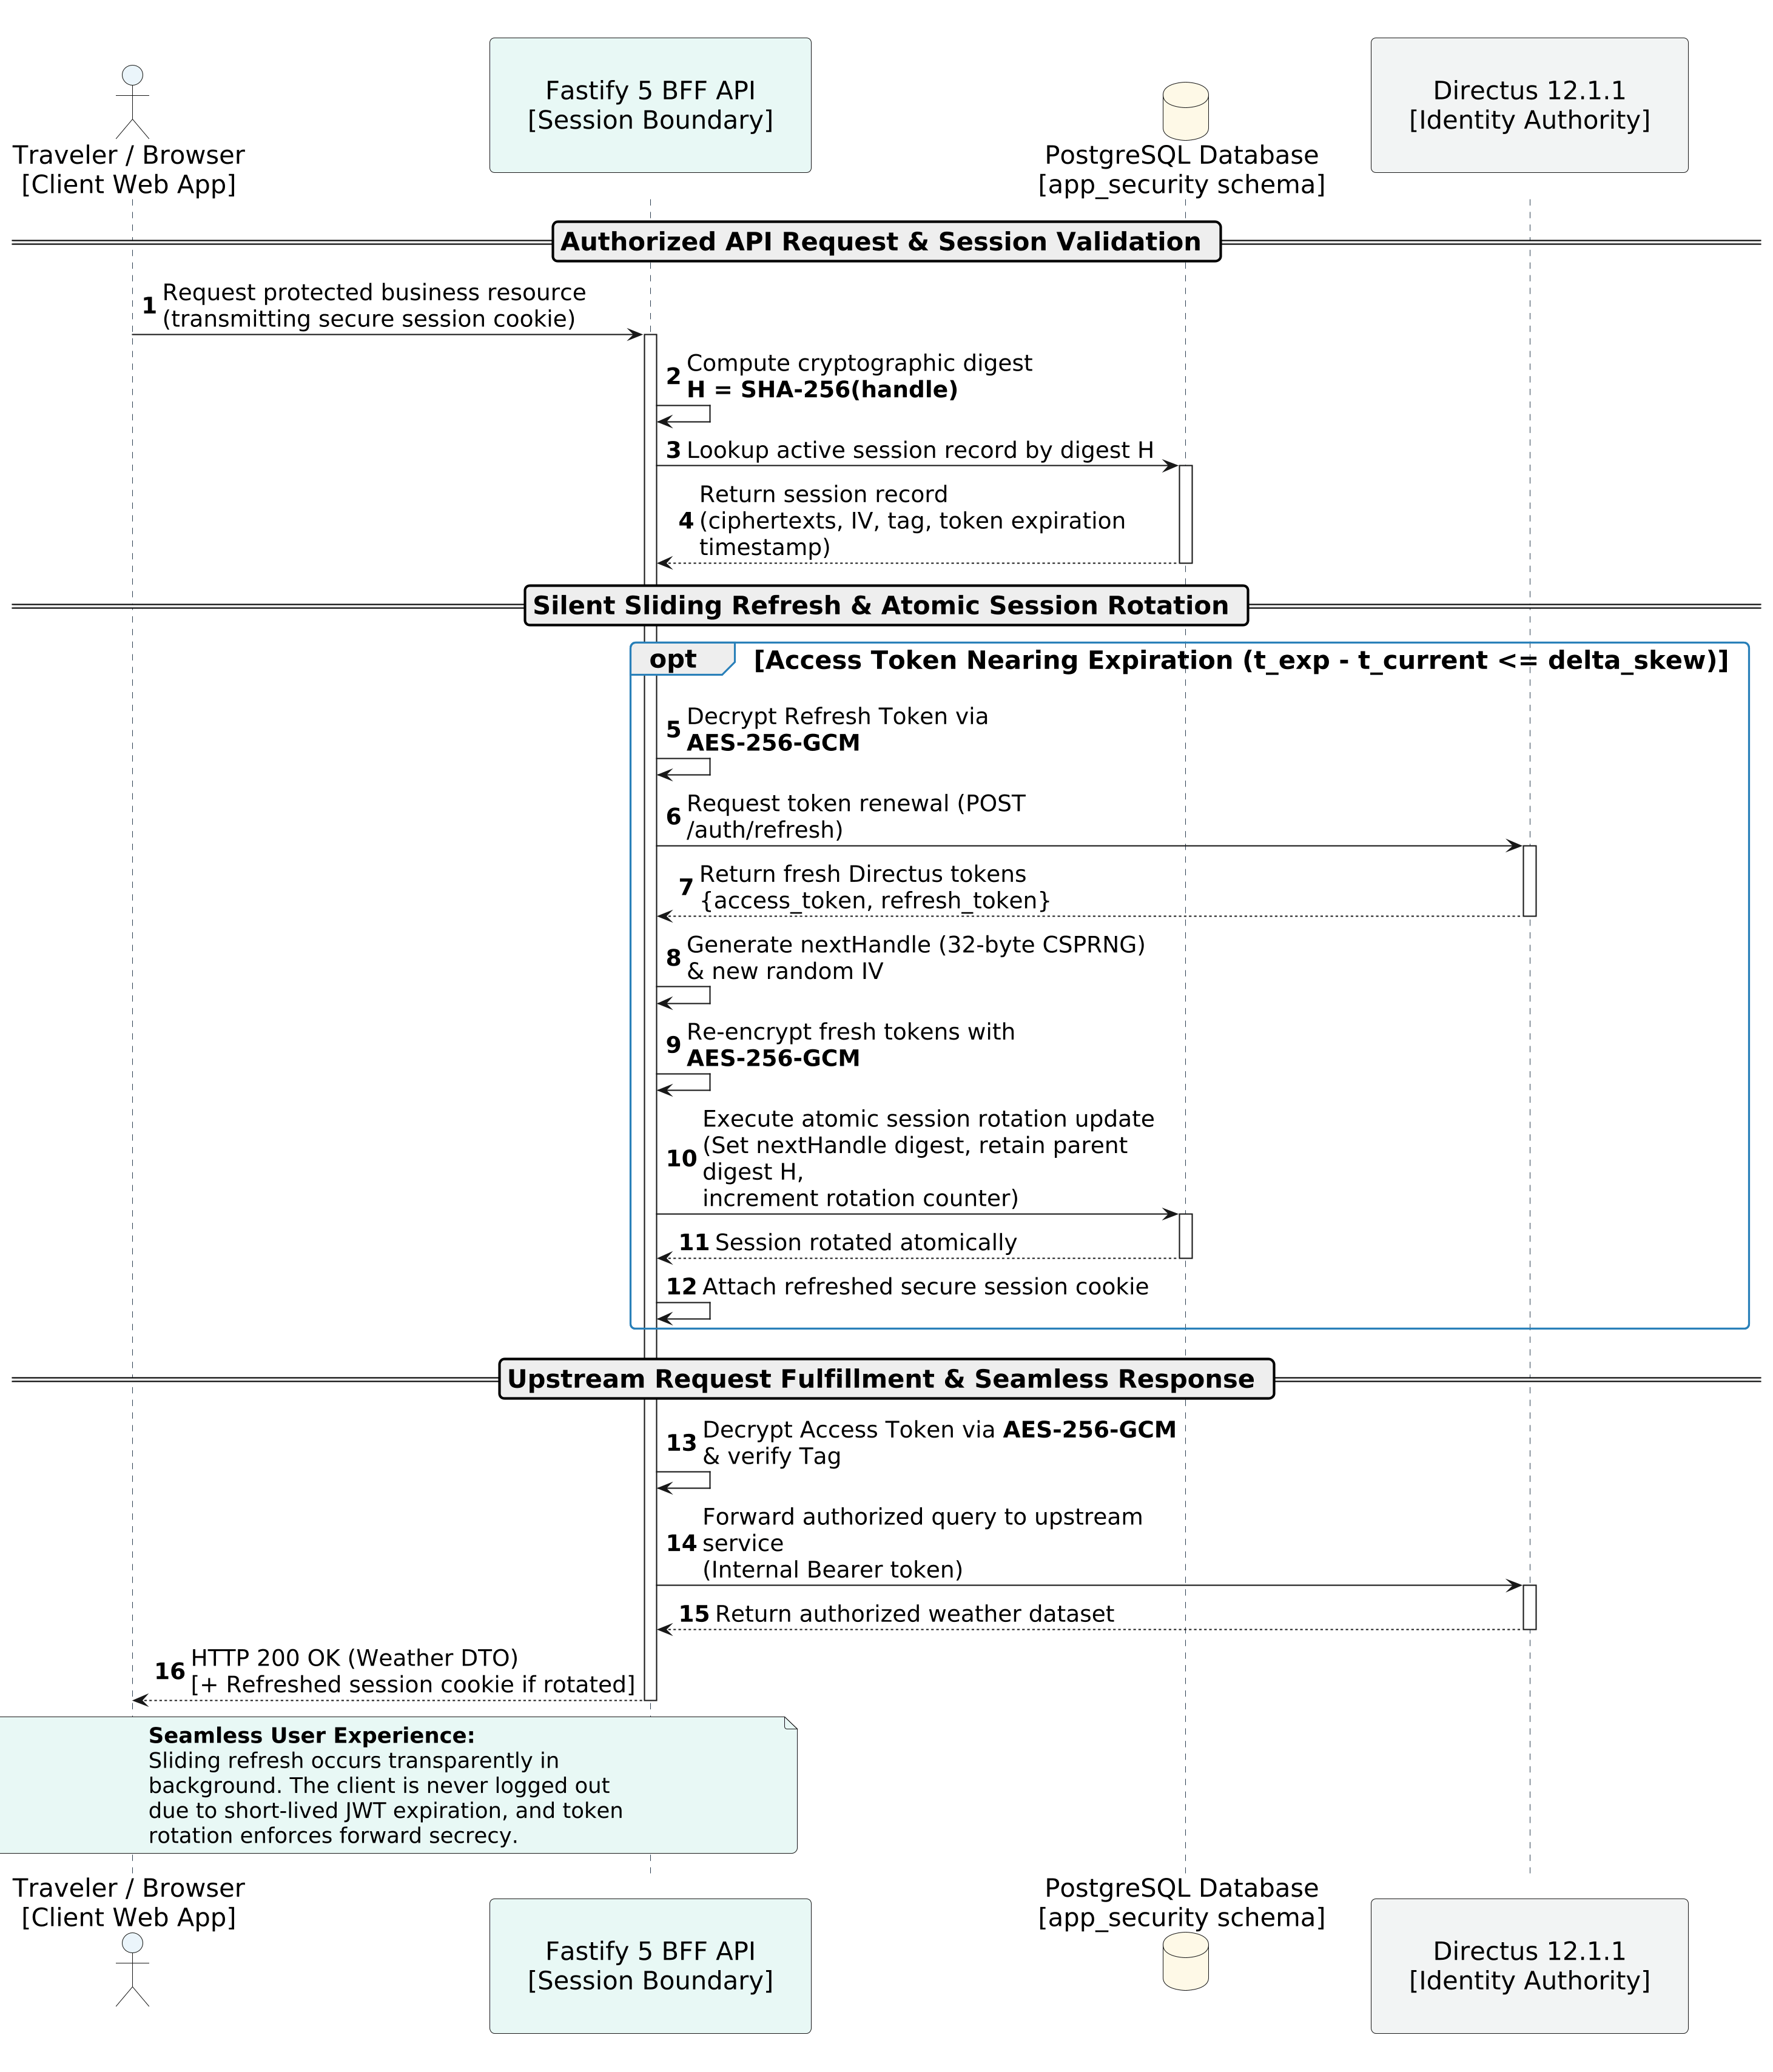
\includegraphics[width=0.92\textwidth, keepaspectratio]{figures/seq_sliding_rotation.png}
\caption[Sequence diagram of session lifecycle (ADR-004) - Phase 2: Sliding Rotation]{Sequence diagram of the secure session lifecycle (ADR-004) (cont.) -- Phase 2: Authorized API request validation and silent sliding rotation (Silent Sliding Refresh).}
\label{fig:seq_auth_lifecycle_p2_en}
\end{figure}

The operational flow of Phase 2 proceeds as follows:
\begin{itemize}
    \item[-] \textit{Step 1 (Cookie interception and digest lookup)}: On incoming client business requests carrying the \texttt{\_\_Host-\allowbreak vnwa\_\allowbreak session} cookie, Fastify extracts handle $h$, computes digest $H = \text{SHA-256}(h)$, and checks the active session table in PostgreSQL (or Redis cache). If no valid unrevoked record exists, Fastify halts execution with HTTP 401 Unauthorized.
    \item[-] \textit{Step 2 (Sliding refresh tolerance window evaluation)}: Fastify evaluates the remaining validity duration of the decrypted Access Token. If the interval until expiration $t_{\text{exp}}$ falls within tolerance window $\Delta t_{\text{skew}}$:
    \begin{equation}
    \label{eq:sliding_skew_en}
    t_{\text{exp}} - t_{\text{current}} \le \Delta t_{\text{skew}}
    \end{equation}
    the backend automatically initiates silent sliding rotation transparently to the user.
    \item[-] \textit{Step 3 (Token renewal and atomic state transition)}: Fastify utilizes key $K_{\text{enc}}$ to decrypt the Refresh Token and invokes Directus to acquire fresh tokens. It then generates next-generation handle $h_{k+1}$ (32-byte CSPRNG) and vector $\text{IV}_{k+1}$. State transition executes atomically via operator $\mathcal{T}_{\text{rotate}}$:
    \begin{equation}
    \label{eq:rotate_session_en}
    \begin{aligned}
    \mathcal{T}_{\text{rotate}}(S_k) \xrightarrow{\text{atomic}} S_{k+1} = \big\langle & \text{SHA-256}(h_{k+1}),\; \mathcal{C}_{k+1}, \\
    & \text{IV}_{k+1},\; \text{Tag}_{k+1},\; t_{\text{exp}, k+1},\; c_k + 1 \big\rangle
    \end{aligned}
    \end{equation}
    while preserving ancestor lineage linkage to detect replay attempts:
    \begin{equation}
    \label{eq:rotate_lineage_en}
    S_{k+1}.\text{ancestor\_hash} = H_k
    \end{equation}
    \item[-] \textit{Step 4 (Grace period retention and request fulfillment)}: Ancestor handle $h_k$ is retained in Redis for a 60-second grace period ($\text{TTL}_{\text{grace}} = 60\text{ s}$) to service in-flight concurrent requests without raising false-positive security exceptions. Fastify decrypts the fresh Access Token, executes the upstream weather query, and dispatches the data payload to the client accompanied by the refreshed session cookie $h_{k+1}$.
\end{itemize}

\subsubsection{Phase 3: Synchronized Revocation and Session Family Annihilation}
Figure~\ref{fig:seq_auth_lifecycle_p3_en} depicts the sequence execution of synchronized event-driven trigger revocation and session family annihilation upon token reuse detection.

\begin{figure}[H]
\ContinuedFloat
\centering
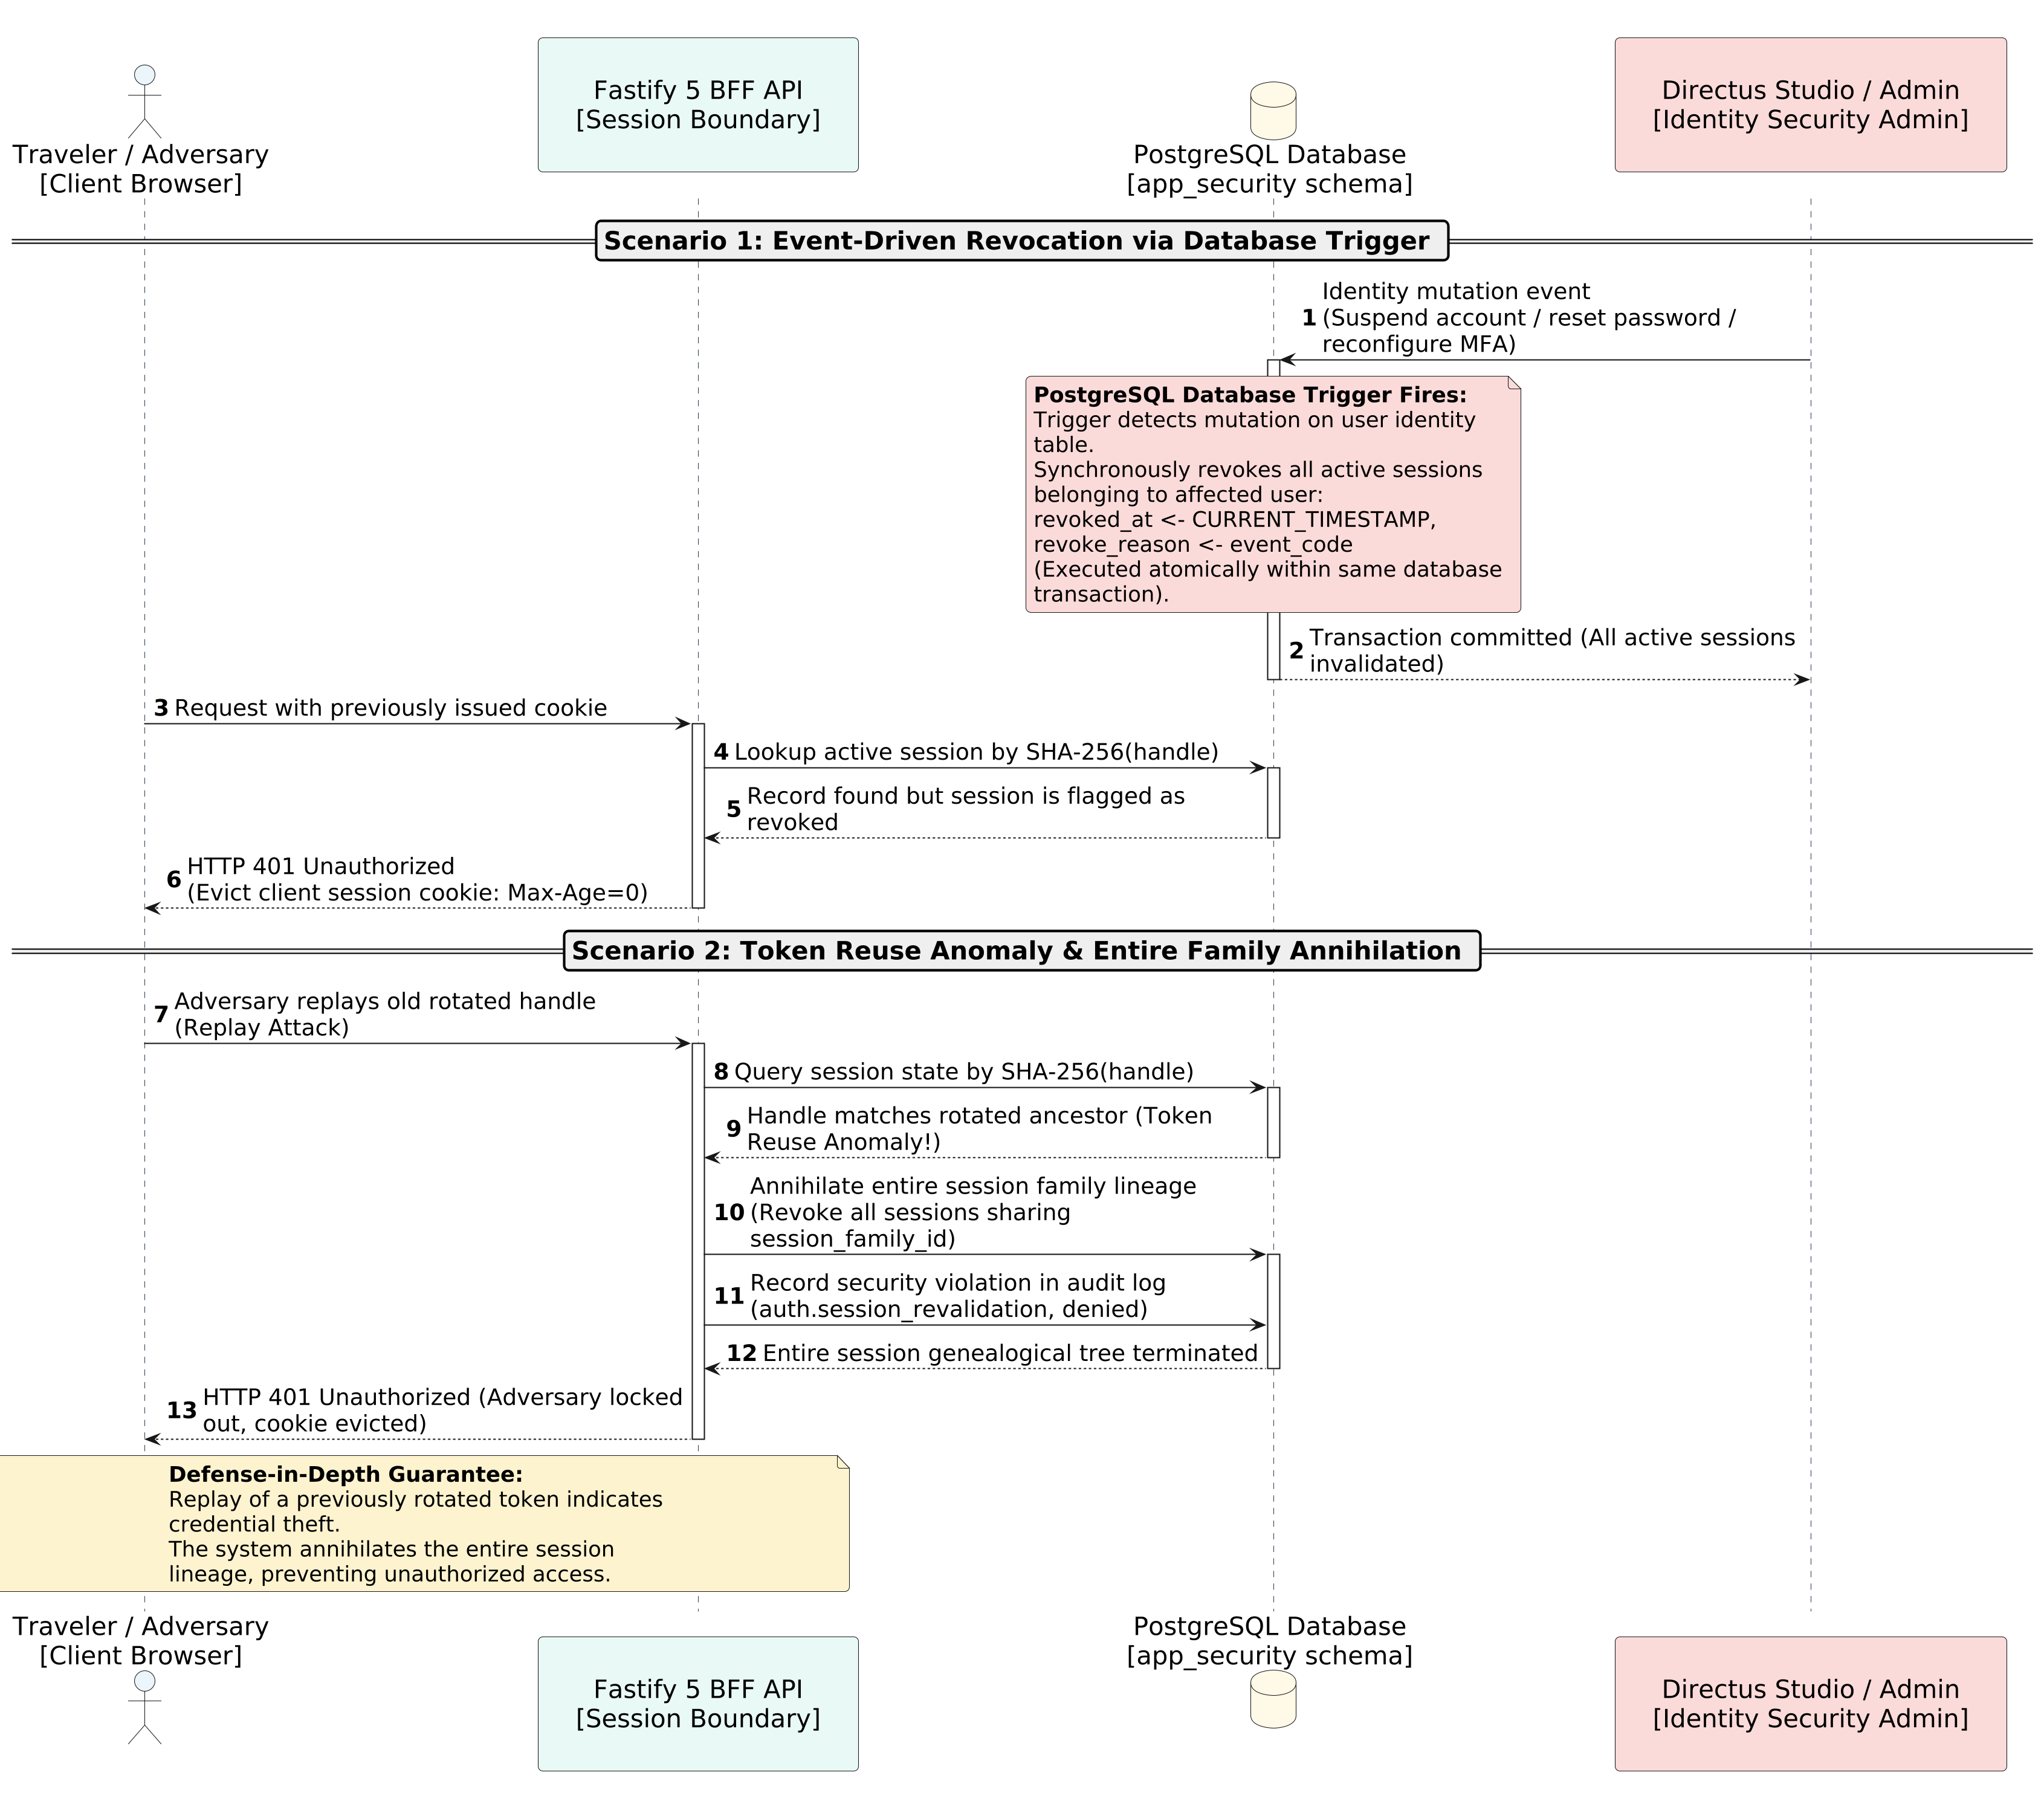
\includegraphics[width=0.92\textwidth, keepaspectratio]{figures/seq_session_revocation.png}
\caption[Sequence diagram of session lifecycle (ADR-004) - Phase 3: Synchronized Revocation]{Sequence diagram of the secure session lifecycle (ADR-004) (cont.) -- Phase 3: Synchronized database trigger revocation and session family annihilation upon token reuse detection.}
\label{fig:seq_auth_lifecycle_p3_en}
\end{figure}

The operational flow of Phase 3 is governed by three rigorous defense mechanisms:
\begin{itemize}
    \item[-] \textit{Scenario 1 (Event-driven database trigger revocation)}: When an administrator suspends an account via Directus Studio, or when a user updates credentials or multi-factor authentication (MFA), an identity mutation event occurs. A database trigger immediately invokes operator $\Phi_{\text{trigger}}$ inside the same ACID transaction:
    \begin{equation}
    \label{eq:trigger_revoke_en}
    \begin{aligned}
    \forall s \in \mathcal{S}, \; (s.\text{user\_id} = u \;\wedge\; s.\text{revoked\_at} = \emptyset) \implies \\
    \Phi_{\text{trigger}}(s) : \begin{cases}
    s.\text{revoked\_at} \leftarrow t_{\text{event}} \\
    s.\text{revoke\_reason} \leftarrow \text{code}_{\text{reason}}
    \end{cases}
    \end{aligned}
    \end{equation}
    where $t_{\text{event}}$ is the transaction timestamp, and $\text{code}_{\text{reason}}$ identifies the mutation cause (\texttt{identity\_}\allowbreak\texttt{password\_}\allowbreak\texttt{changed}, \texttt{identity\_}\allowbreak\texttt{status\_}\allowbreak\texttt{changed}, \texttt{identity\_}\allowbreak\texttt{role\_}\allowbreak\texttt{changed}, \texttt{identity\_}\allowbreak\texttt{mfa\_}\allowbreak\texttt{changed}, or \texttt{identity\_}\allowbreak\texttt{deleted}). All active sessions of user $u$ across all physical devices are immediately revoked.
    \item[-] \textit{Scenario 2 (Token reuse detection and session family annihilation)}: If an adversary presents an expired handle already rotated beyond the 60-second grace window, Fastify detects a hash collision with ancestor record $S.\text{ancestor\_hash}$. Fastify flags an active token theft and invokes family annihilation operator $\Psi_{\text{annihilate}}$:
    \begin{equation}
    \label{eq:family_revoke_en}
    \begin{aligned}
    \forall s \in \mathcal{S}, \; (s.\text{family\_id} = F_{\text{target}}) \implies \\
    \Psi_{\text{annihilate}}(s) : \begin{cases}
    s.\text{revoked\_at} \leftarrow t_{\text{detection}} \\
    s.\text{revoke\_reason} \leftarrow \text{`token\_reuse\_detected'}
    \end{cases}
    \end{aligned}
    \end{equation}
    All descendant tokens within the session family are purged from Redis and marked revoked in PostgreSQL, and an urgent security alert is appended to audit logs.
    \item[-] \textit{Scenario 3 (Voluntary termination and automated maintenance)}: Upon explicit logout (\texttt{POST /auth/logout}), Fastify sets \texttt{revoked\_at} in PostgreSQL, removes Redis cache entries, and clears client cookies by issuing \texttt{Max-Age=0}. A background database retention routine periodically prunes revoked session records exceeding regulatory retention intervals.
\end{itemize}

\section{Background Integration Worker and Resilience Patterns (ADR-001)}
\label{sec:worker_resilience_adr001}

\subsection{Fault Domain Isolation Between Background Tasks and APIs}
During operational meteorological ingestion, polling third-party external APIs (such as WeatherAPI) exhibits non-trivial failure probabilities stemming from transit congestion, remote provider outages, or rate quota exhaustion. Furthermore, harvesting data across Vietnam's 63 provinces on 15-to-30-minute cadences induces substantial network I/O and normalization workloads.

Co-locating these ingestion pipelines within the primary user-facing API process or relying on long-running Directus Flows risks blocking the Node.js event loop, precipitating severe API latency degradation and catastrophic cascading failures. Therefore, in adherence to architectural decision ADR-001, all ingestion, normalization, metric calculation, and cache hydration workloads are completely isolated inside an autonomous daemon named Integration Worker.

\subsection{Distributed Database Leasing and Concurrency Control}
To prevent redundant ingestion cycles when scaling worker nodes horizontally across multiple containers or cluster nodes, the platform implements distributed database leasing backed by the PostgreSQL table \texttt{weather\_worker\_leases}.

The leasing mechanism enforces atomic acquisition with expiration:
\begin{itemize}
    \item[-] At the start of an ingestion cycle, a candidate worker attempts an atomic conditional upsert (\texttt{INSERT ... ON CONFLICT DO UPDATE}) on the lease lock record. Acquisition succeeds only if no worker currently holds the lease or the existing lease timestamp has lapsed.
    \item[-] Lease tenure is configured by parameter \texttt{WEATHER\_}\allowbreak\texttt{WORKER\_}\allowbreak\texttt{LEASE\_}\allowbreak\texttt{DURATION\_MS} ($120,000\text{ ms}$).
    \item[-] Throughout active data ingestion and normalization, the worker dispatches heartbeat pings every 30,000 milliseconds (\texttt{HEARTBEAT\_INTERVAL\_MS} ($30,000\text{ ms}$)) to extend lease validity.
    \item[-] If a worker crashes or suffers network partition, heartbeat signals cease. Once the 120-second lease TTL lapses, the lease expires cleanly without distributed deadlock, allowing standby workers to assume ingestion duties seamlessly.
\end{itemize}

\subsection{Circuit Breaker Pattern and Adaptive Backoff}
To preserve provider quota budgets and maintain local platform stability during upstream outages, the Integration Worker incorporates a three-state Circuit Breaker pattern:
\begin{itemize}
    \item[-] \textit{Closed State (CLOSED)}: WeatherAPI requests execute normally while consecutive failure counters are continuously tracked.
    \item[-] \textit{Open State (OPEN)}: When consecutive network failures (HTTP 5xx, HTTP 429, or timeouts exceeding \texttt{TIMEOUT\_MS} ($8,000\text{ ms}$)) reach \texttt{CIRCUIT\_FAILURE\_}\allowbreak\texttt{THRESHOLD} ($3$ attempts), the circuit trips to Open. In this state, outgoing calls are immediately short-circuited locally without placing network load on upstream servers.
    \item[-] \textit{Half-Open State (HALF-OPEN)}: Upon expiry of \texttt{CIRCUIT\_RESET\_MS} ($60,000\text{ ms}$), the breaker transitions to Half-Open and issues a single probe request. If successful, the circuit resets to Closed; otherwise, it immediately re-enters Open and restarts the backoff timer.
\end{itemize}

For transient errors, the worker applies exponential backoff with full jitter. Delay duration for retry attempt $k$ is calculated as:
\begin{equation}
\label{eq:backoff_jitter_en}
t_{\text{delay}}(k) = \min\left(t_{\max}, \; t_{\text{base}} \cdot 2^{k-1}\right) \cdot \left(1 + r_{\text{jitter}} \cdot \mathcal{U}(-1, 1)\right)
\end{equation}
with base backoff $t_{\text{base}} = 5,000\text{ ms}$, maximum backoff $t_{\max} = 60,000\text{ ms}$, jitter ratio $r_{\text{jitter}} = 0.2$, and $\mathcal{U}(-1, 1)$ representing a continuous uniform random variable on $[-1, 1]$. This stochastic jitter prevents thundering herd contention across station retry cycles.

\subsection{Meteorological Data Freshness Lifecycle and Safe States}
Observations ingested by the worker undergo normalization to WMO-No. 8 units and SHA-256 integrity digest generation before insertion into \texttt{weather\_}\allowbreak\texttt{observations}. Simultaneously, \texttt{weather\_forecasts} records are updated and Redis cache keys are refreshed.

Persisted weather observations are governed by a three-tier freshness state model to ensure the validity and safety of route hazard evaluations:
\begin{itemize}
    \item[-] \textit{Fresh State}: Observation latency $\tau \le 60\text{ minutes}$ from station observation timestamp. Fully validated and representative of actual atmospheric conditions; ingested directly into the route risk scoring engine.
    \item[-] \textit{Aging State}: Observation latency $60 < \tau \le 180\text{ minutes}$. Data remains consumable for corridor routing computations, but client interfaces display an aging timestamp advisory to inform travelers.
    \item[-] \textit{Stale State}: When observation latency $\tau > 180\text{ minutes}$ (or weather station disconnection exceeds 3 hours). Under Fail-Safe engineering principles, stale telemetry is rejected for hazard derivation and automatically mapped to the \texttt{Unknown} risk tier (neutral gray \#9CA3AF), guaranteeing users are alerted to missing field observations rather than receiving unverified safety assurances.
\end{itemize}

Figure~\ref{fig:seq_ingestion_en} illustrates the end-to-end background ingestion lifecycle, covering distributed lease acquisition, circuit breaker evaluation, data normalization, and cache hydration.

\begin{figure}[H]
\centering
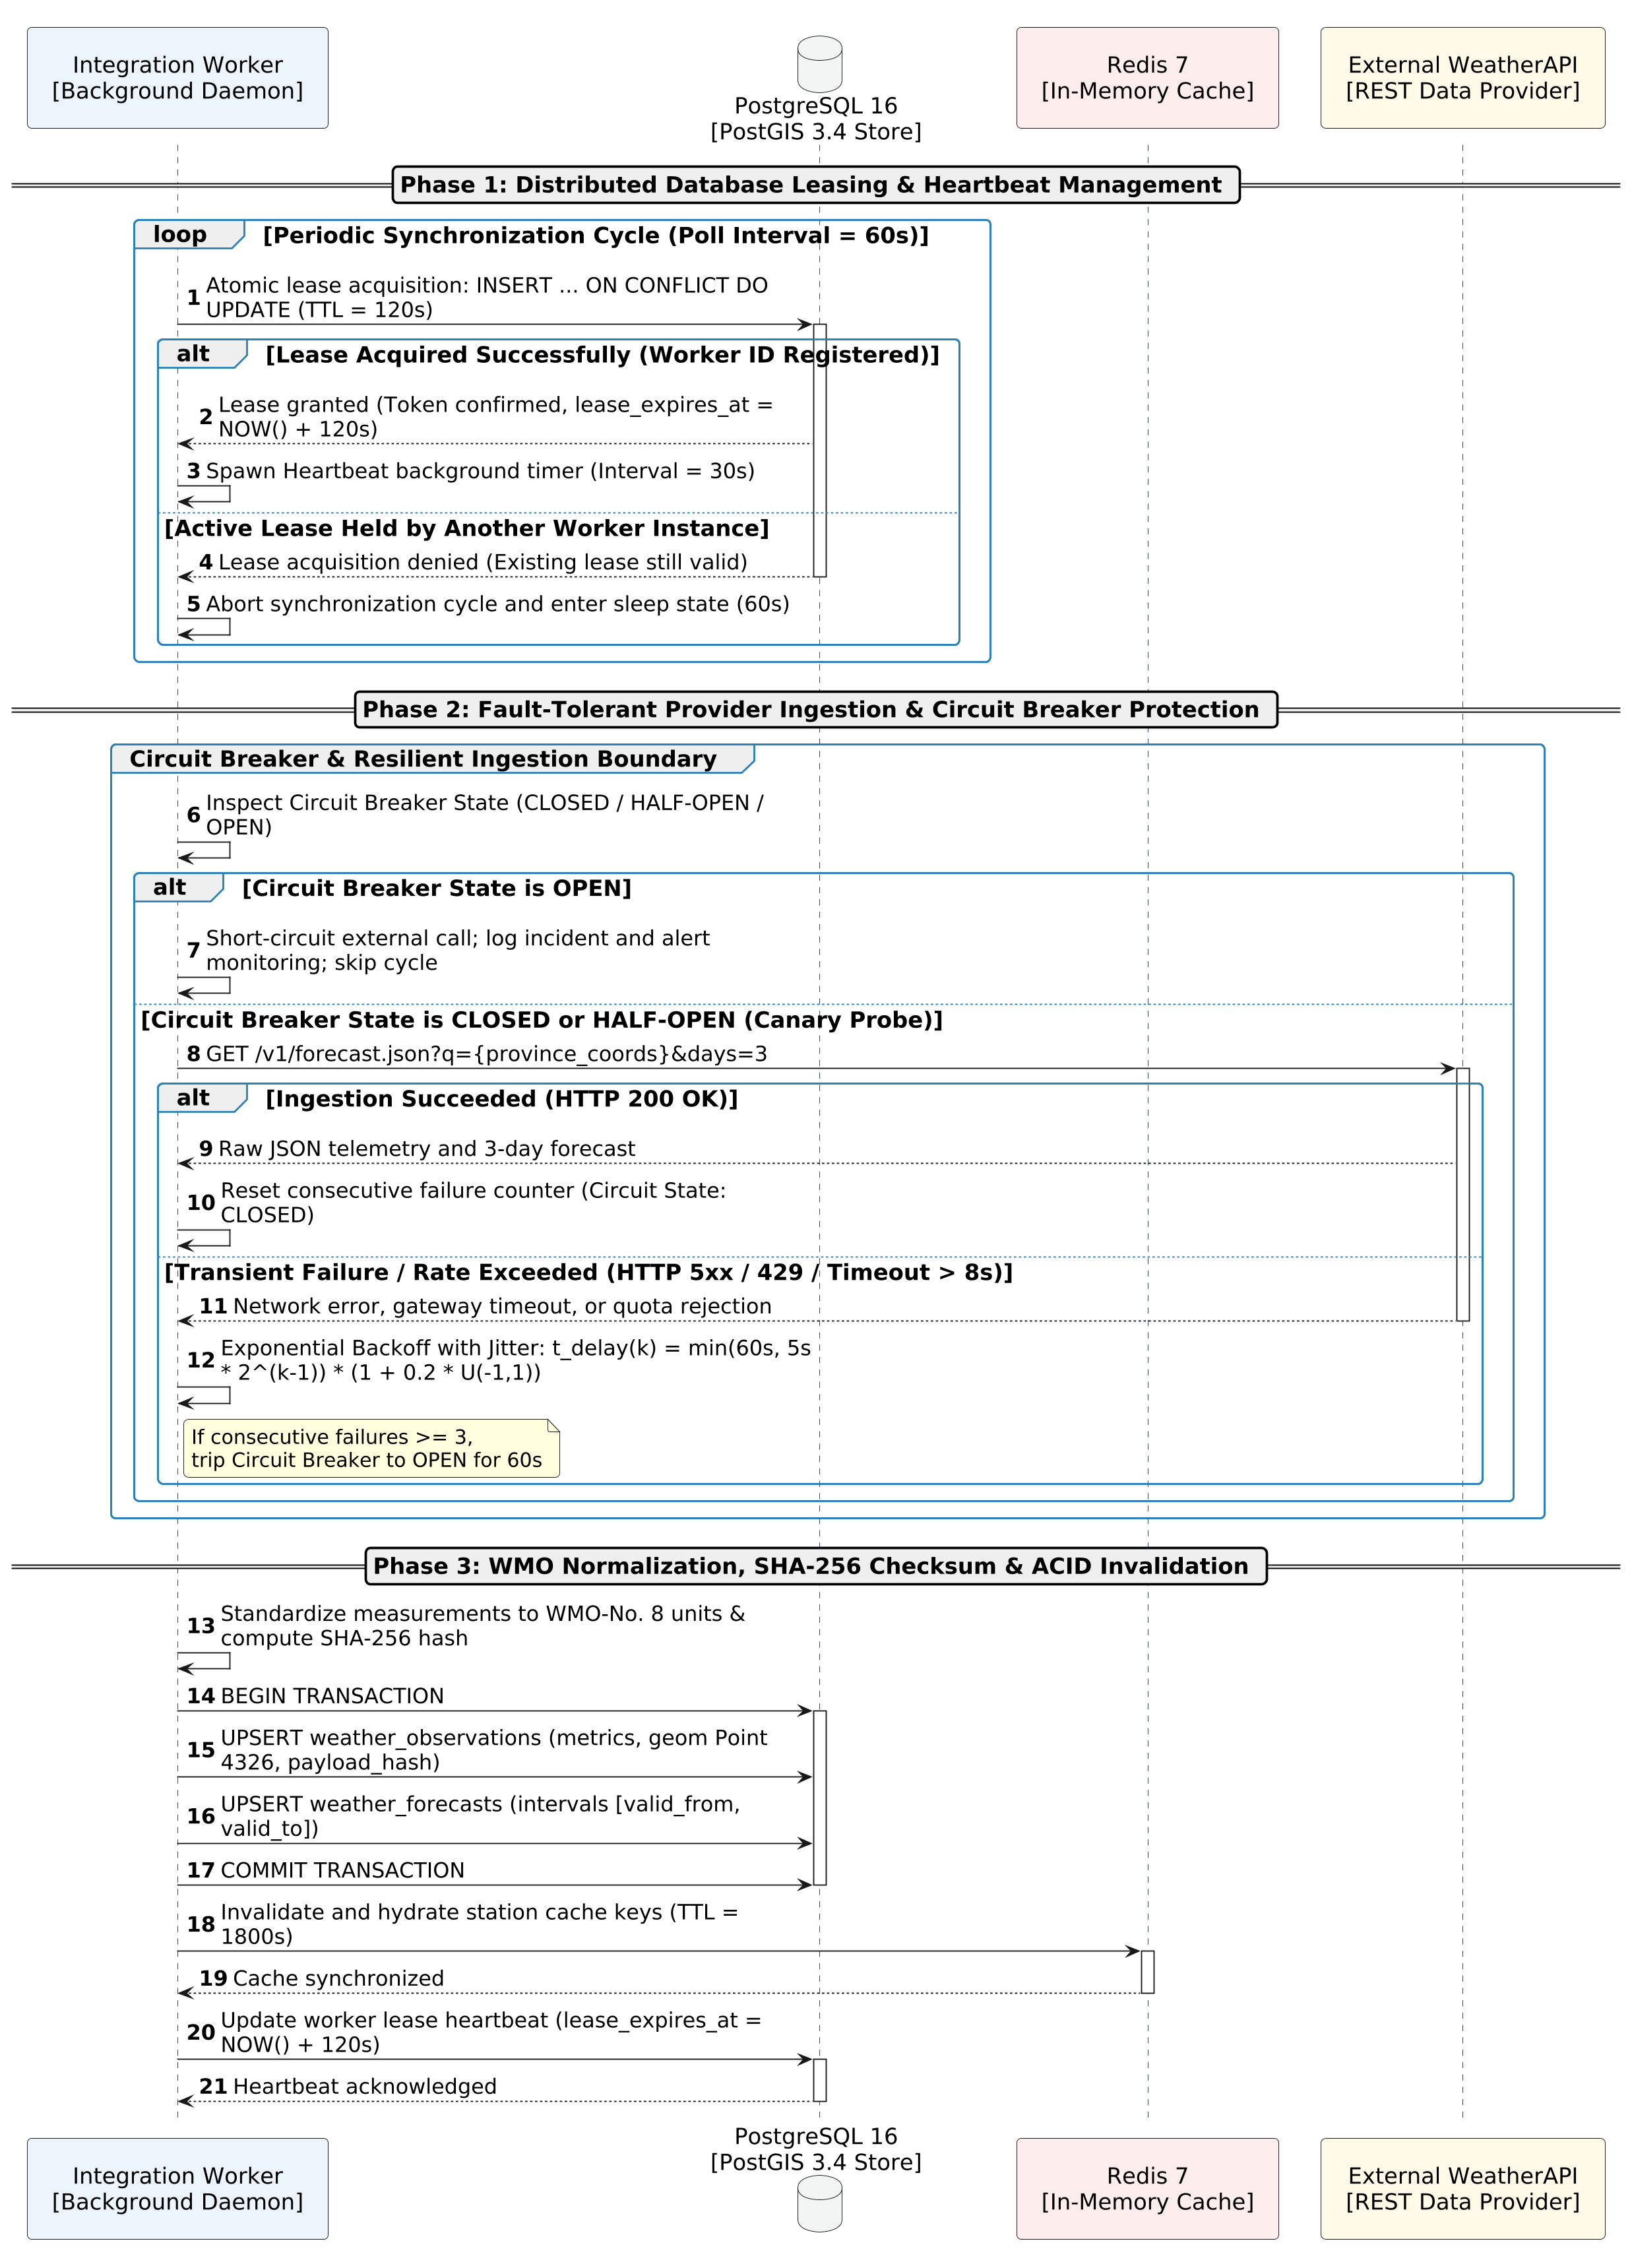
\includegraphics[width=0.90\textwidth, height=0.65\textheight, keepaspectratio]{figures/seq_ingestion.png}
\caption[Sequence diagram of background meteorological ingestion (ADR-001)]{Sequence diagram of background meteorological ingestion, distributed leasing, and circuit breaker protection (ADR-001).}
\label{fig:seq_ingestion_en}
\end{figure}

The operational execution flow of the autonomous Integration Worker encompasses three foundational phases:
\begin{itemize}
    \item[-] \textit{Phase 1: Distributed Database Leasing and Heartbeat Management}:
    Every 60 seconds (the polling interval), the worker attempts atomic, exclusive lease acquisition on PostgreSQL table \texttt{weather\_worker\_leases} via \texttt{INSERT ... ON CONFLICT DO UPDATE WHERE lease\_expires\_at < NOW()}. This atomic condition guarantees that exactly one active worker executes ingestion across distributed containers. Upon acquiring the lease (TTL = $120,000\text{ ms}$), the worker spawns an asynchronous heartbeat timer at 30-second intervals to periodically renew the lease horizon (\texttt{lease\_expires\_at} $= \text{NOW}() + 120\text{s}$). If an active lease is already held by another worker instance, acquisition is denied and the candidate worker enters a 60-second sleep state without resource contention.
    \item[-] \textit{Phase 2: Fault-Tolerant Provider Ingestion and Circuit Breaker Protection}:
    Prior to dispatching external network requests across Vietnam's 63 provinces, the worker inspects its internal Circuit Breaker state. If the circuit is \texttt{OPEN}, the worker short-circuits execution, logging an alert and skipping ingestion to preserve API quotas and relieve external server pressure. If the circuit is \texttt{CLOSED} or \texttt{HALF-OPEN}, the worker dispatches \texttt{GET /v1/forecast.json?q=\{province\_coords\}\&days=3} to WeatherAPI. Upon receiving HTTP 200 OK, consecutive failure counters are reset to zero. In the event of transient upstream failures (HTTP 5xx, HTTP 429 quota exhaustion, or request timeouts exceeding 8 seconds), the worker applies exponential backoff with stochastic jitter $t_{\text{delay}}(k)$ per Equation~\eqref{eq:backoff_jitter_en}. If consecutive failures reach the threshold of 3, the circuit breaker trips to \texttt{OPEN} for 60 seconds.
    \item[-] \textit{Phase 3: WMO Normalization, SHA-256 Checksum and ACID Invalidation}:
    Raw JSON telemetry is transformed into standardized WMO-No. 8 units (Celsius temperatures, meters per second wind speeds, and millimeter precipitation depths). The worker computes a SHA-256 cryptographic digest over the canonical observation payload to prevent duplicate inserts. Next, the worker opens an explicit database transaction (\texttt{BEGIN TRANSACTION}) and performs atomic \texttt{UPSERT} operations into \texttt{weather\_observations} (storing surface measurements with Point 4326 geometries and timestamps) and \texttt{weather\_forecasts} (storing discretized temporal validity intervals), subsequently committing the transaction (\texttt{COMMIT TRANSACTION}). Upon successful persistent commit, the worker invalidates and hydrates Redis cache keys (\texttt{TTL = 1800s}) to ensure low-latency API retrieval, while renewing the lease heartbeat timestamp in PostgreSQL.
\end{itemize}

\section{PostGIS Spatial Database Schema and Entity-Relationship Architecture}
\label{sec:postgis_erd_schema}

\subsection{Tiered Database Domain Architecture}
The VietForecast persistent store operates on PostgreSQL 16 enhanced with the PostGIS 3.4 spatial extension. The database schema is partitioned into modular functional domains:
\begin{itemize}
    \item[-] \textit{Security and Session Domain} (\texttt{app\_security}): Contains \texttt{app\_security.}\allowbreak\texttt{sessions} storing AES-256-GCM encrypted token envelopes and \texttt{app\_security.audit\_events} capturing immutable audit logs.
    \item[-] \textit{Administrative and Spatial Domain} (\texttt{administrative}): Contains \texttt{administrative\_}\allowbreak\texttt{units} detailing Vietnam's administrative tree (Country $\rightarrow$ 63 Provinces $\rightarrow$ Districts $\rightarrow$ Communes) with \texttt{MultiPolygon} boundaries, and \texttt{locations} cataloging observation stations, landmarks, and transportation nodes with \texttt{geometry(Point, 4326)}.
    \item[-] \textit{Meteorological Data Domain} (\texttt{weather}): Contains \texttt{weather\_}\allowbreak\texttt{providers}, \texttt{weather\_}\allowbreak\texttt{observations} storing surface time-series metrics with SHA-256 checksums, \texttt{weather\_}\allowbreak\texttt{forecasts} holding interval validity ranges $[t_{\text{start}}, t_{\text{end}}]$, and \texttt{weather\_}\allowbreak\texttt{worker\_}\allowbreak\texttt{leases} coordinating distributed worker locks.
    \item[-] \textit{Risk Rule and Route Domain} (\texttt{risk\_route}): Houses \texttt{risk\_}\allowbreak\texttt{rule\_}\allowbreak\texttt{sets} and \texttt{risk\_}\allowbreak\texttt{rules} under Maker-Checker governance, \texttt{risk\_}\allowbreak\texttt{assessments} with audit evidence, alongside \texttt{route\_}\allowbreak\texttt{requests}, \texttt{route\_}\allowbreak\texttt{options}, and \texttt{route\_}\allowbreak\texttt{samples} holding LineString geometries and spatiotemporal sample waypoints.
\end{itemize}

\subsection{Spatial Query Optimization with GiST Indexes}
In highway corridor hazard evaluation, the platform must query all meteorological observation stations situated within an $r_{\text{corridor}} = 15\text{ km}$ buffer corridor surrounding a travel itinerary spanning hundreds of kilometers. Evaluating geodetic distance across entire tables via sequential scans incurs $O(M \cdot N)$ complexity (where $M$ is the route sample count and $N$ is total observation records), causing latency spikes of several seconds.

PostGIS 3.4 overcomes this limitation by implementing Generalized Search Tree (GiST) indexing over all geometry columns. GiST structures spatial features as hierarchical bounding box trees (Minimum Bounding Box -- BBOX). The spatial engine executes a two-tier filtering strategy:
\begin{itemize}
    \item[-] \textit{Rough Pass (Bounding Box Filter)}: The query engine evaluates intersection between the bounding box of the route buffer corridor $G_{\text{corridor}} = \text{ST\_Buffer}(\mathcal{L}, r_{\text{corridor}})$ and candidate station bounding boxes:
    \begin{equation}
    \label{eq:spatial_bbox_filter_en}
    \text{BBOX}(o.\text{geom}) \cap \text{BBOX}(G_{\text{corridor}}) \ne \emptyset
    \end{equation}
    Traversing the balanced GiST index requires only $O(\log N)$ operations, filtering out over 95\% of distant stations without expensive spherical trigonometry.
    \item[-] \textit{Exact Pass}: PostGIS applies exact ellipsoidal geodesic distance computations (\texttt{ST\_DWithin} on \texttt{geography} data types) exclusively to candidates surviving the rough pass:
    \begin{equation}
    \label{eq:spatial_exact_filter_en}
    d_{\text{geodetic}}(o.\text{geom}, \mathcal{L}) \le r_{\text{corridor}} \quad \text{with } \tau(o) \le 180\text{ minutes}
    \end{equation}
    ensuring mathematical precision under the WGS84 ellipsoid in under 15 milliseconds. The concrete spatial GiST indexing parameters and two-tier corridor query specifications are detailed in Table~\ref{tab:gist_query_spec_en} in Chapter~\ref{ch:implementation}.
\end{itemize}

\subsection{Standardized Entity-Relationship Diagram and Governance Constraints}
Figure~\ref{fig:erd_database_en} depicts the Entity-Relationship Diagram (ERD) of the VietForecast core data architecture, specifying primary keys, foreign key linkages, and referential constraints.

\begin{figure}[H]
\centering
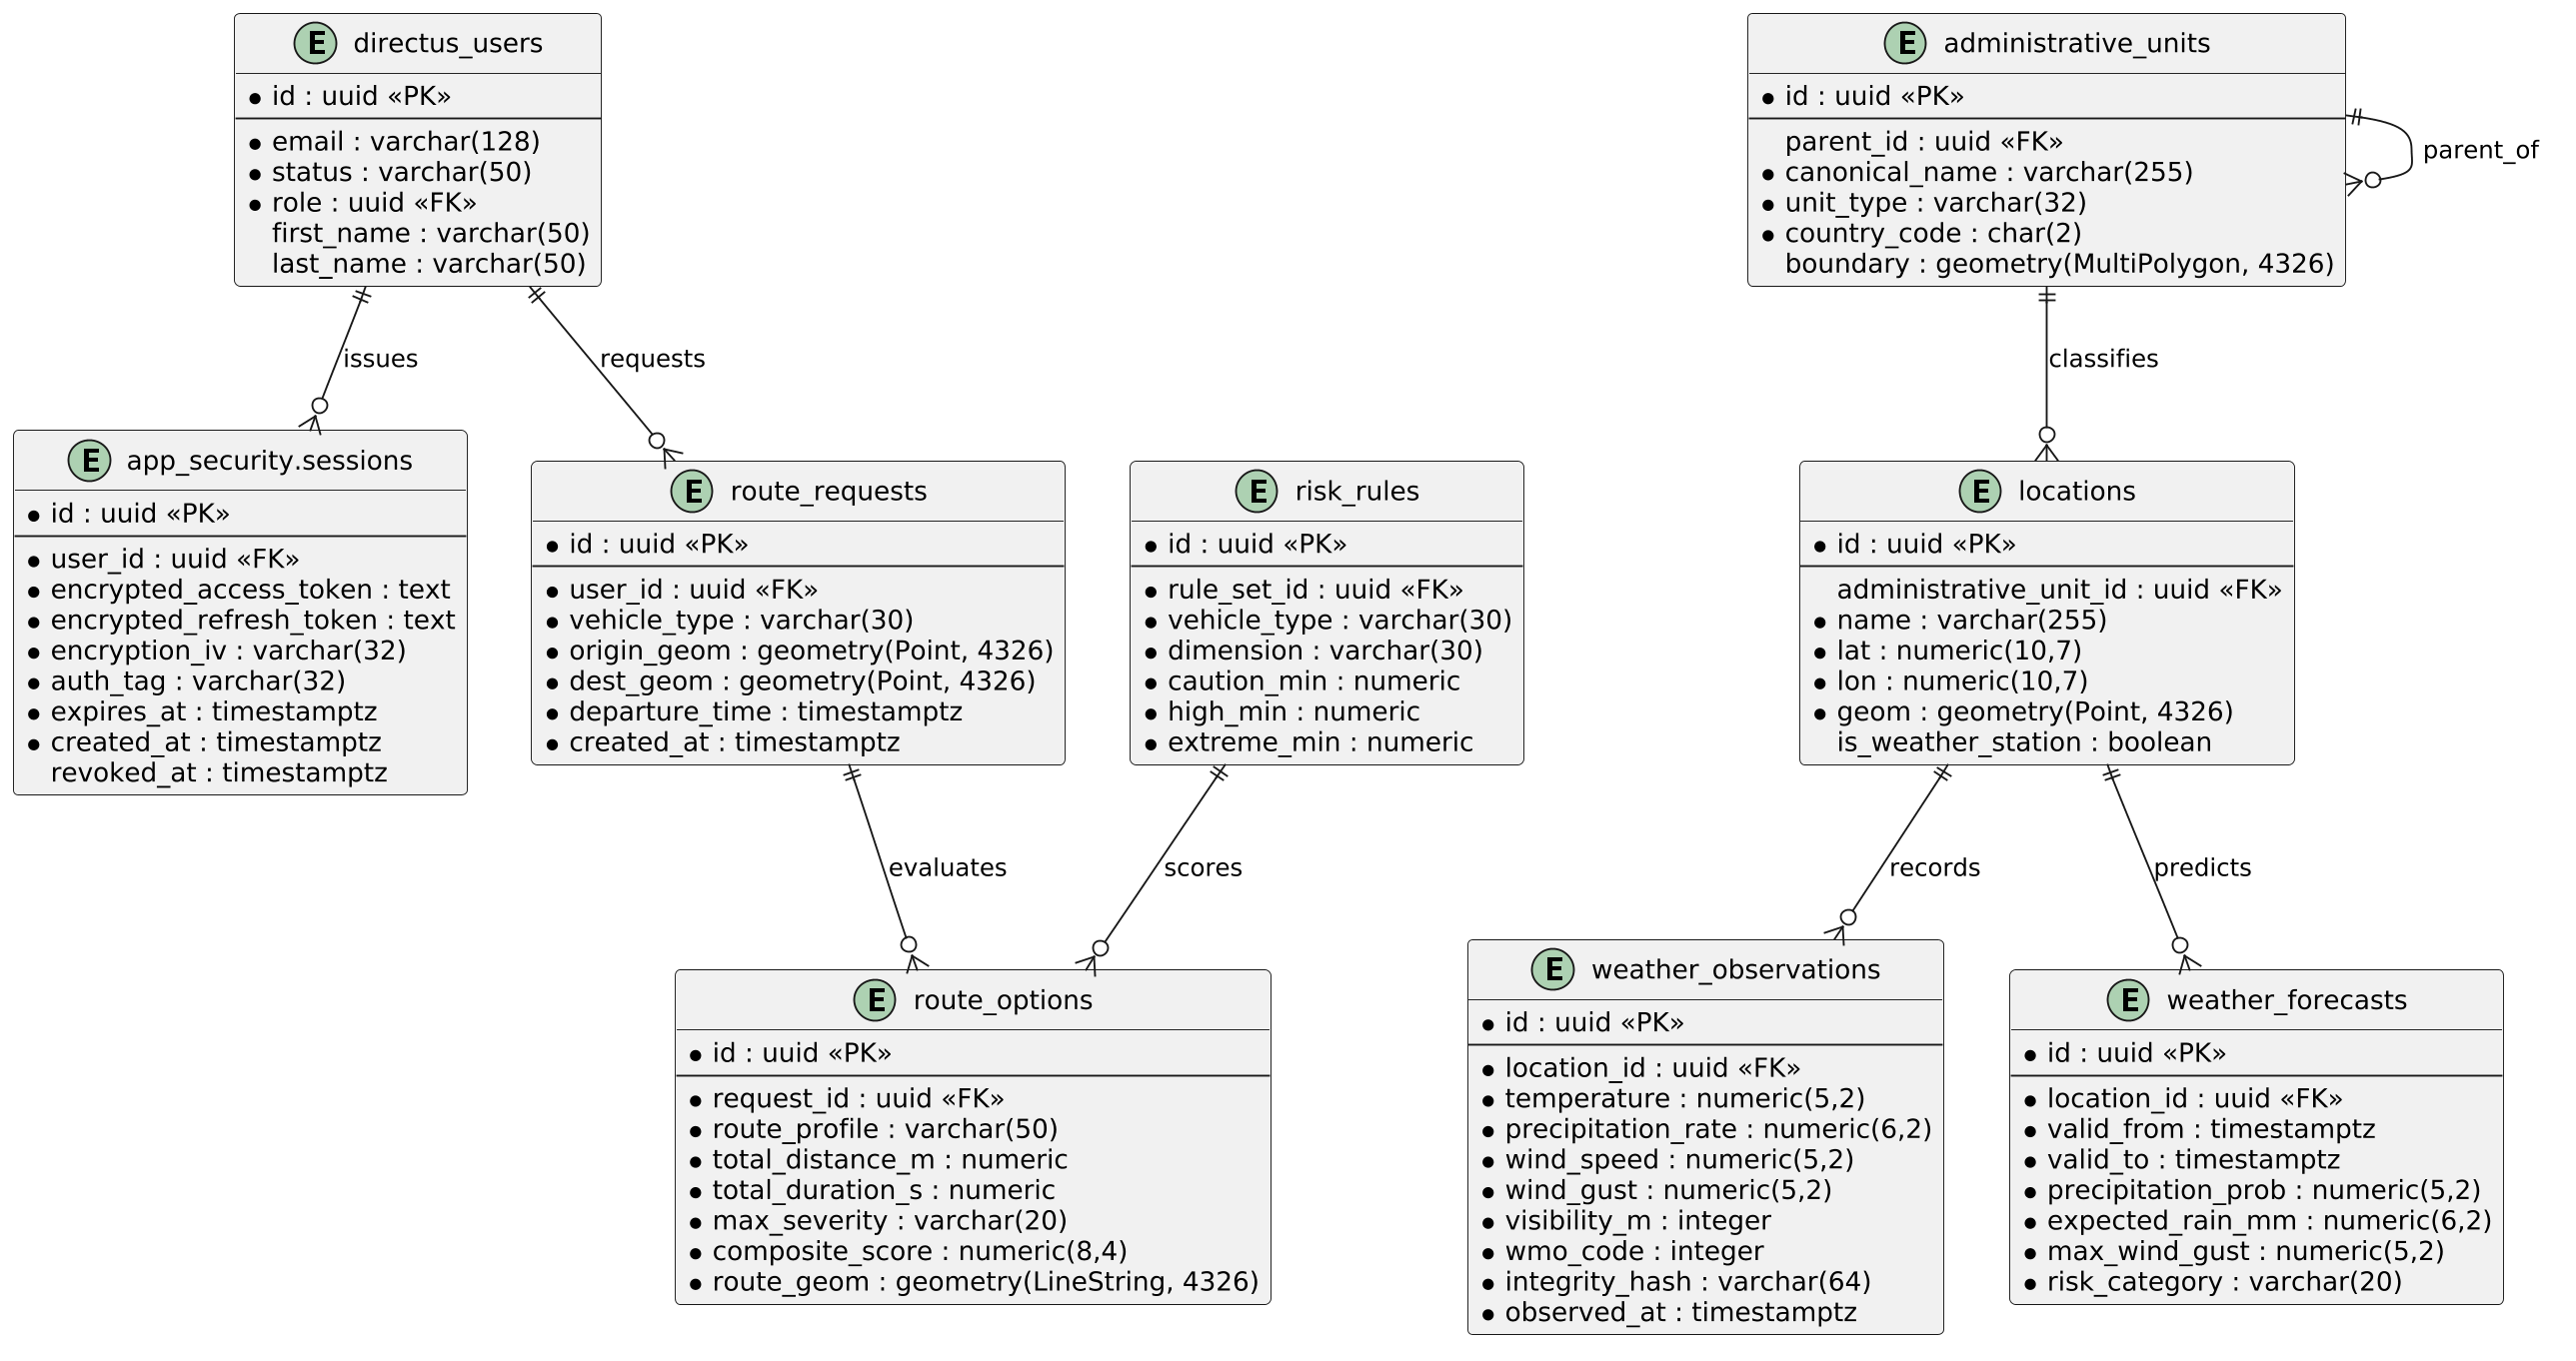
\includegraphics[width=0.95\textwidth, height=0.62\textheight, keepaspectratio]{figures/erd_database.png}
\caption[Entity-Relationship Diagram (ERD) of VietForecast]{Entity-Relationship Diagram (ERD) illustrating spatial data structures, identity security, and risk rule governance in VietForecast.}
\label{fig:erd_database_en}
\end{figure}

The \texttt{directus\_}\allowbreak\texttt{users} entity serves as the authoritative identity anchor across the platform, binding active security sessions in \texttt{app\_}\allowbreak\texttt{security.}\allowbreak\texttt{sessions} to historical routing queries in \texttt{route\_}\allowbreak\texttt{requests}. Two advanced governance mechanisms enforce structural integrity:
\begin{itemize}
    \item[-] \textit{Maker-Checker Governance for Risk Rules}: Risk rule sets within \texttt{risk\_}\allowbreak\texttt{rule\_}\allowbreak\texttt{sets} transition sequentially across: \texttt{draft}, \texttt{review}, \texttt{approved}, \texttt{published}, and \texttt{retired}. Database trigger \texttt{app\_}\allowbreak\texttt{governance.}\allowbreak\texttt{guard\_}\allowbreak\texttt{risk\_}\allowbreak\texttt{rule\_}\allowbreak\texttt{mutation()} prohibits modifications or deletions of child rules in \texttt{risk\_}\allowbreak\texttt{rules} once a set departs \texttt{draft}, ensuring historical hazard judgments remain immutable and deterministic.
    \item[-] \textit{Immutable Security Audit Trail}: All administrative mutations regarding credentials, access roles, or threshold parameters automatically emit records into \texttt{app\_}\allowbreak\texttt{security.}\allowbreak\texttt{audit\_}\allowbreak\texttt{events} via \texttt{SECURITY DEFINER} triggers, preventing unauthorized tampering with security history.
\end{itemize}

\section{Multi-Objective Route Risk Evaluation and Balancing Engine}
\label{sec:route_risk_engine}

\subsection{Spatiotemporal Modeling and Route Corridor Discretization}
The primary objective of the route risk evaluation engine is transforming discrete weather observations into actionable travel guidance for motorists.

The platform queries route geometries from the road routing engine (OSRM), acquiring three alternative itineraries: Fastest, Shortest, and Alternative, each defined as a GeoJSON LineString accompanied by total distance $D$ and nominal travel duration $T$. The engine discretizes each polyline into a sequence of sample waypoints $p_i = (\phi_i, \lambda_i)$ under dual spatial and temporal constraints: inter-sample spatial separation $\Delta s \le 5\text{ km}$ and temporal advance $\Delta t \le 15\text{ minutes}$, computed from the nominal velocity $\bar{v} = D / T$.

The Fastify API queries PostGIS using \texttt{ST\_DWithin} to aggregate weather stations and forecast grids within a 15 km corridor around each waypoint $p_i$, interpolating atmospheric conditions at expected arrival time $t_i$.

\subsection{Vehicle-Differentiated Hazard Threshold Matrix}
The risk engine cross-references meteorological parameters at each waypoint $p_i$ against a six-dimensional hazard ruleset ($R_{\text{rain}}$, $R_{\text{wind}}$, $R_{\text{temp}}$, $R_{\text{vis}}$, $R_{\text{storm}}$, $R_{\text{alert}}$). Waypoint hazard severity $S(p_i)$ follows the Max-Severity Aggregation principle:
\begin{equation}
\label{eq:max_severity_aggregation_en}
S(p_i) = \max_{d \in \mathcal{D}} R_d(p_i, v)
\end{equation}
where $\mathcal{D} = \{\text{rain}, \text{wind}, \text{temp}, \text{vis}, \text{storm}, \text{alert}\}$ denotes the dimension set, $v \in \{\text{motorcycle}, \text{car}\}$ denotes vehicle type, and $R_d \in \{0, 1, 2, 3\}$ corresponds to \texttt{Unknown} (0), \texttt{Low} (1), \texttt{Caution} (2), and \texttt{High} (3).

Table~\ref{tab:vehicle_risk_matrix_en} delineates the vehicle-differentiated activation thresholds calibrated to Vietnamese road transport safety norms.

\begin{table}[H]
\centering
\small
\caption[Vehicle-differentiated weather hazard activation matrix]{Vehicle-differentiated weather hazard activation matrix (RISK-001, RISK-002).}
\label{tab:vehicle_risk_matrix_en}
\begin{tabularx}{\textwidth}{l >{\raggedright\arraybackslash}p{2.8cm} X X}
\toprule
\textbf{Hazard Dimension} & \textbf{Metric \& Unit} & \textbf{Caution Threshold} & \textbf{High Hazard Threshold} \\
\midrule
Precipitation ($R_{\text{rain}}$) & Rainfall rate (mm/h) & 
Motorcycle: $10 \le r < 25$ \newline Car: $15 \le r < 35$ & 
Motorcycle: $r \ge 25$ \newline Car: $r \ge 35$ \\
\addlinespace
Wind gust ($R_{\text{wind}}$) & Wind gust speed (km/h) & 
Motorcycle: $25 \le w < 40$ \newline Car: $45 \le w < 60$ & 
Motorcycle: $w \ge 40$ \newline Car: $w \ge 60$ \\
\addlinespace
Visibility ($R_{\text{vis}}$) & Horizontal visibility (m) & 
Motorcycle: $1,000 \le v < 2,000$ \newline Car: $500 \le v < 1,000$ & 
Motorcycle: $v < 1,000$ \newline Car: $v < 500$ \\
\addlinespace
Temperature ($R_{\text{temp}}$) & Surface temperature ($^\circ\text{C}$) & 
Motorcycle: $36$--$38^\circ\text{C}$ hoặc $10$--$13^\circ\text{C}$ \newline Car: $38$--$40^\circ\text{C}$ hoặc $5$--$8^\circ\text{C}$ & 
Motorcycle: $> 38^\circ\text{C}$ hoặc $< 10^\circ\text{C}$ \newline Car: $> 40^\circ\text{C}$ hoặc $< 5^\circ\text{C}$ \\
\addlinespace
Thunderstorm ($R_{\text{storm}}$) & WMO convective activity & 
Distant storm or cumulonimbus & 
Direct thunderstorm or hail \\
\addlinespace
Severe Alert ($R_{\text{alert}}$) & National disaster tier & 
Disaster Risk Level 1--2 & 
Disaster Risk Level 3+ \\
\bottomrule
\end{tabularx}
\end{table}

\subsection{Balanced Multi-Objective Route Optimization Function}
The system scores candidate routes utilizing a normalized multi-objective scalarization objective:
\begin{equation}
\label{eq:route_balanced_score_en}
Score_{\text{balanced}} = w_{\text{risk}} \cdot \hat{S}_{\text{route}} + w_{\text{time}} \cdot \hat{T} + w_{\text{dist}} \cdot \hat{D}
\end{equation}
with default weights $w_{\text{risk}} = 0.5$, $w_{\text{time}} = 0.3$, and $w_{\text{dist}} = 0.2$. Normalized route hazard $\hat{S}_{\text{route}} = \frac{1}{K} \sum_{k=1}^K S(p_k) / 3$, distance $\hat{D} = D / \max(D)$, and travel duration $\hat{T} = T / \max(T)$ map to $[0, 1]$. The lowest-scoring corridor receives the Weather-Safer Recommended designation, balancing transit efficiency against severe weather exposure.

\subsection{Route Hazard Evaluation Pipeline and Sequence Diagram}
Figure~\ref{fig:seq_route_risk_en} details the comprehensive sequence flow of multi-alternative hazard evaluation upon user route submission via the MapLibre GL frontend.

\begin{figure}[H]
\centering
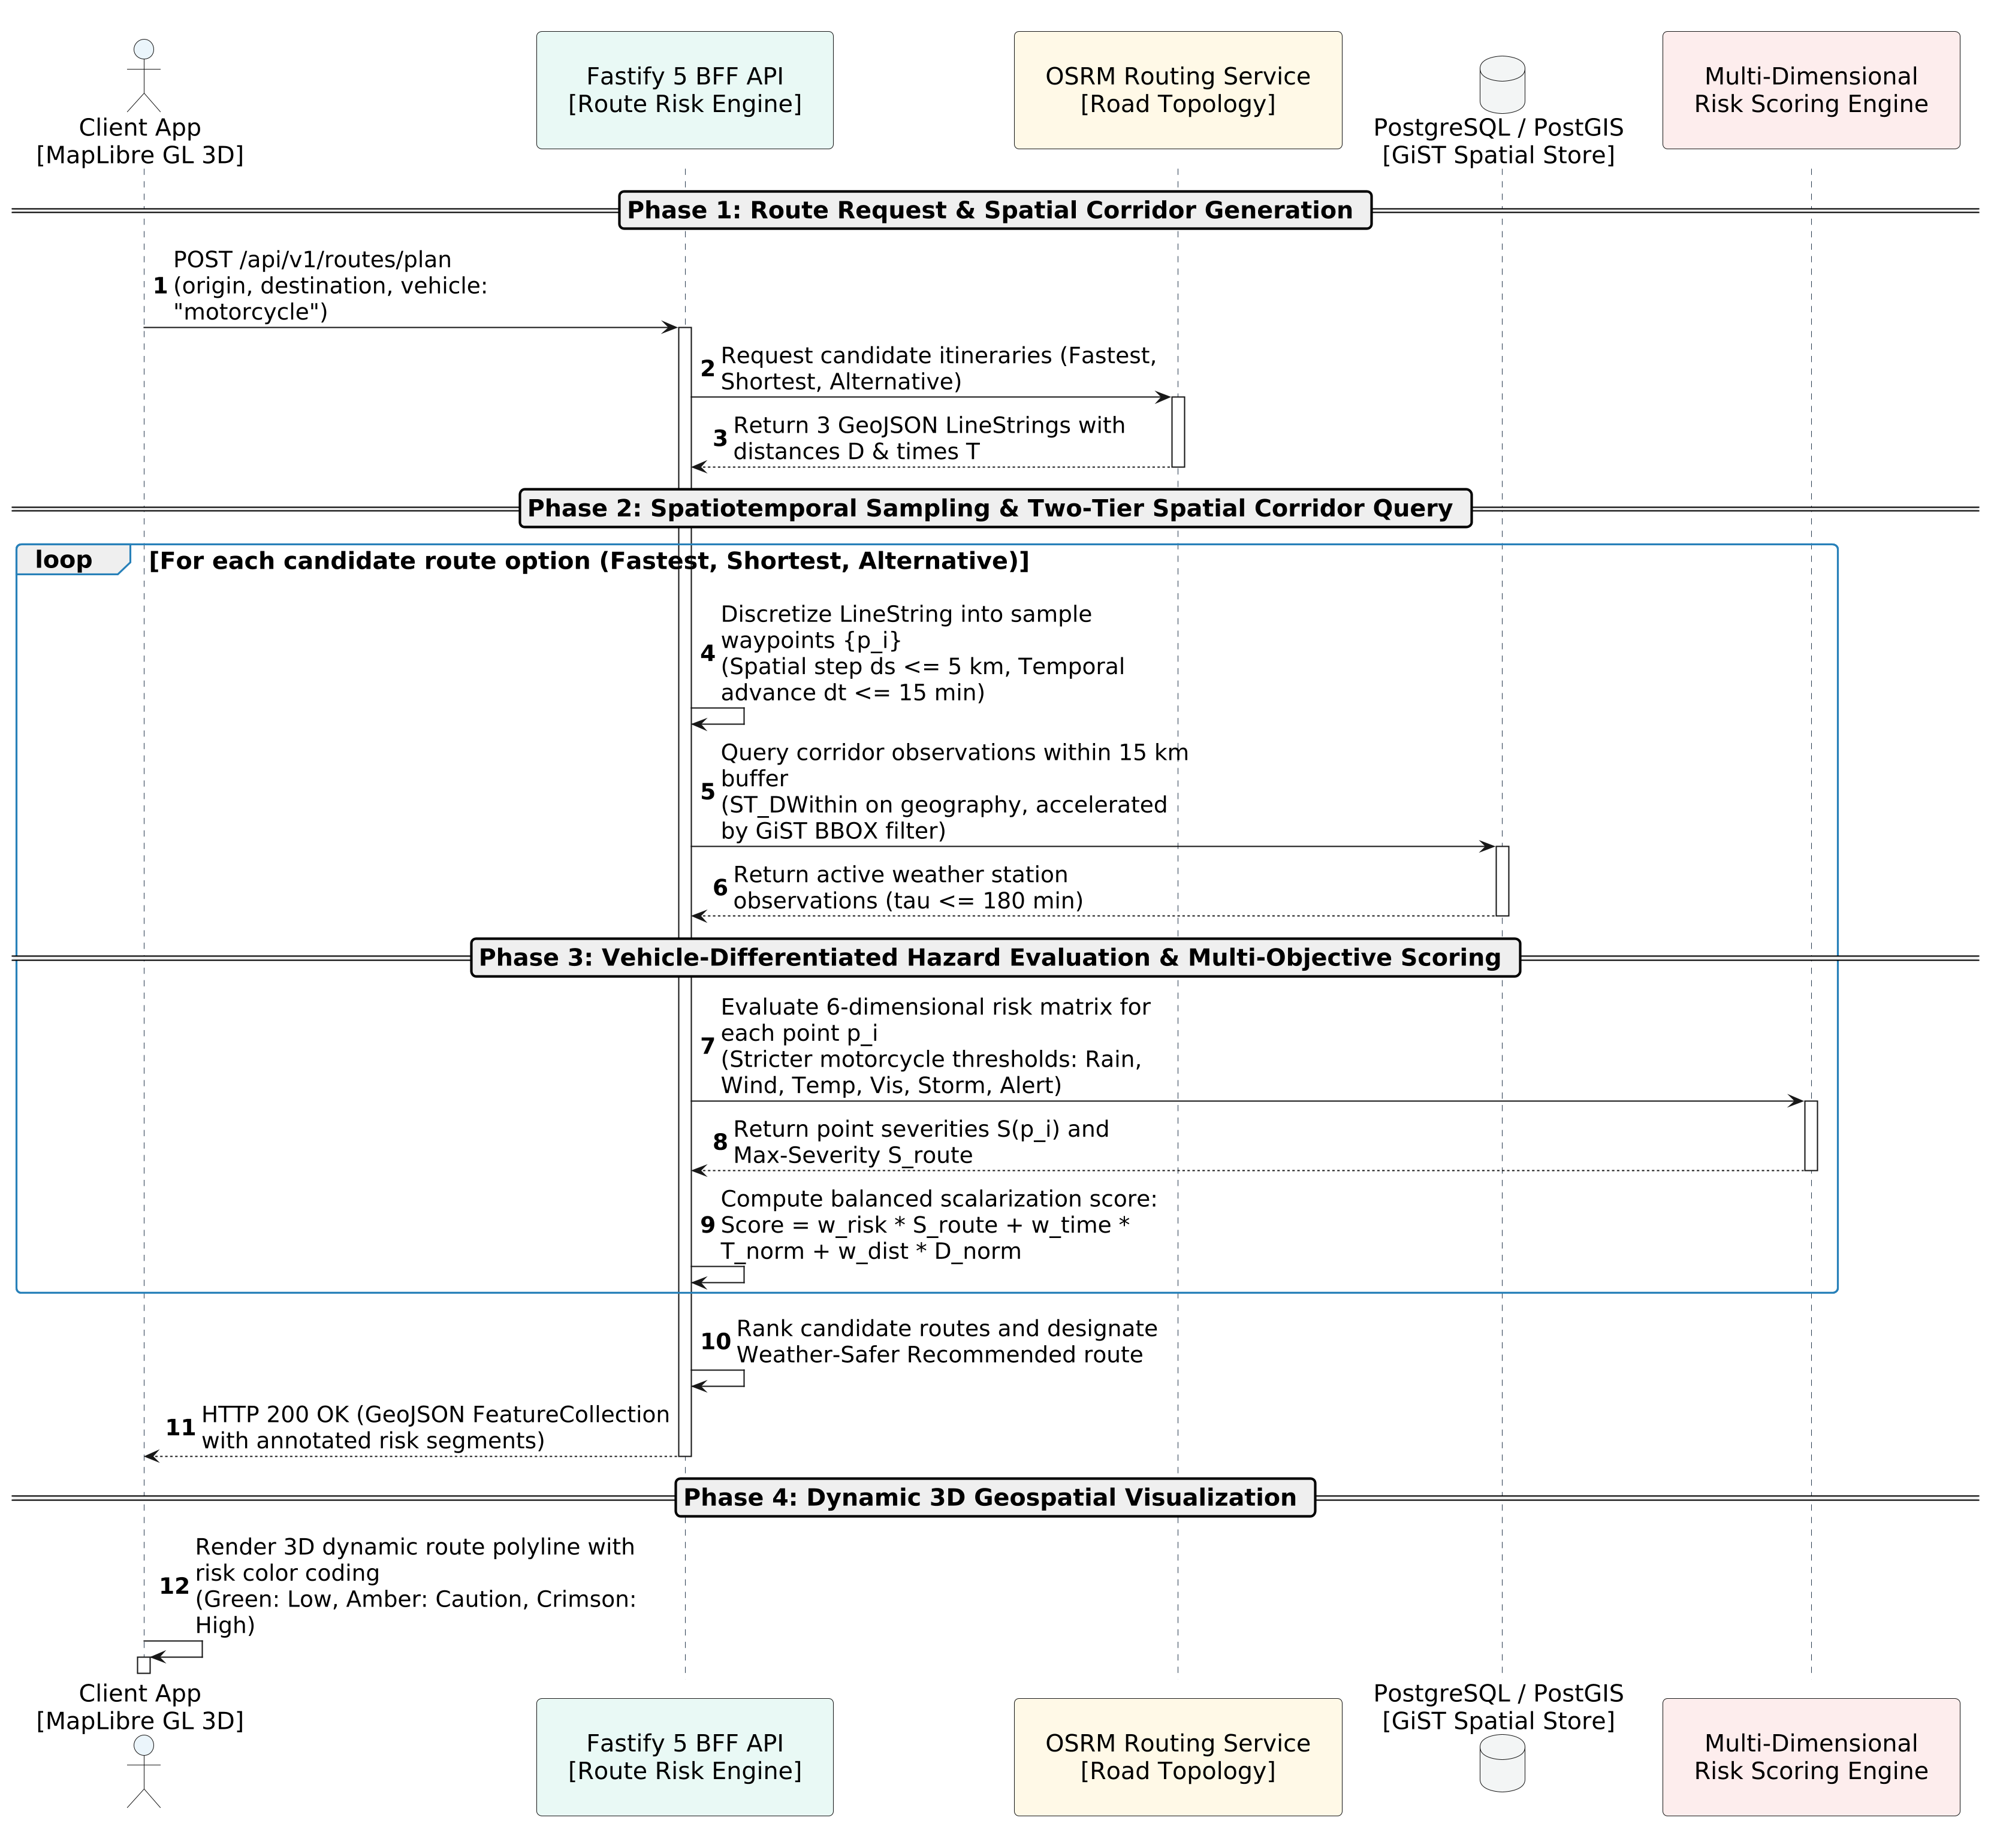
\includegraphics[width=0.95\textwidth, keepaspectratio]{figures/seq_route_risk.png}
\caption[Sequence diagram of multi-objective route hazard evaluation]{Sequence diagram of multi-objective route risk evaluation, spatiotemporal sampling, and 3D map visualization.}
\label{fig:seq_route_risk_en}
\end{figure}

The operational flow of the route risk evaluation engine executes across four foundational phases:
\begin{itemize}
    \item[-] \textit{Phase 1: Route request dispatch and candidate corridor extraction}:
    The client single page application dispatches a \texttt{POST /api/v1/routes/plan} request with trip parameters (origin, destination, and vehicle profile: \texttt{motorcycle} or \texttt{car}) to Fastify API. Fastify delegates road network routing to OSRM, extracting three alternative routes: Fastest, Shortest, and Alternative. Each candidate route is returned as a GeoJSON LineString accompanied by total transit distance $D$ and nominal travel duration $T$.
    \item[-] \textit{Phase 2: Spatiotemporal sampling and two-tier spatial corridor query}:
    For each candidate itinerary, the engine discretizes the continuous LineString into a sequence of discrete check waypoints $p_i = (\phi_i, \lambda_i)$ constrained by spatial spacing $\Delta s \le 5\text{ km}$ and temporal steps $\Delta t \le 15\text{ minutes}$ (derived from nominal velocity $\bar{v} = D / T$).
    At each waypoint $p_i$, Fastify executes an optimized PostGIS spatial query using \texttt{ST\_DWithin}. The GiST 2D spatial index accelerates rough-pass filtering over bounding boxes in $O(\log N)$ time, after which exact ellipsoidal geodesic distance computations are applied over the WGS84 ellipsoid to aggregate active weather stations and forecast records within an $r_{\text{corridor}} = 15\text{ km}$ buffer having observation freshness $\tau \le 180\text{ minutes}$.
    \item[-] \textit{Phase 3: Vehicle-differentiated hazard evaluation and multi-objective scoring}:
    Atmospheric observations collected at each waypoint $p_i$ are evaluated against the six-dimensional hazard ruleset: Precipitation ($R_{\text{rain}}$), Wind gust ($R_{\text{wind}}$), Surface temperature ($R_{\text{temp}}$), Visibility ($R_{\text{vis}}$), Convective storms ($R_{\text{storm}}$), and Disaster alert tier ($R_{\text{alert}}$). Waypoint hazard severity $S(p_i)$ is resolved via the Max-Severity Aggregation principle $S(p_i) = \max_{d \in \mathcal{D}} R_d(p_i, v)$ per Equation~\eqref{eq:max_severity_aggregation_en}. For motorcycle riders, hazard thresholds are tightened by over 30\% relative to passenger cars to reflect heightened vulnerability (Table~\ref{tab:vehicle_risk_matrix_en}).
    The system calculates the scalarized multi-objective balanced score $Score_{\text{balanced}}$ according to Equation~\eqref{eq:route_balanced_score_en}, balancing route hazard exposure ($\hat{S}_{\text{route}}$), transit duration ($\hat{T}$), and geographical distance ($\hat{D}$). The lowest-scoring route receives the Weather-Safer Recommended designation.
    \item[-] \textit{Phase 4: GeoJSON serialization and dynamic 3D geospatial rendering}:
    Fastify returns an HTTP 200 OK response containing a GeoJSON FeatureCollection with segmented route geometries color-coded by hazard severity: green (\texttt{Low}), amber (\texttt{Caution}), and crimson (\texttt{High}). MapLibre GL 4 leverages WebGL hardware acceleration to render the 3D terrain mesh and dynamic route polyline, allowing motorists to inspect hazard hotspots along their itinerary interactively.
\end{itemize}

\section{Grounded Conversational Weather AI Engine}
\label{sec:grounded_ai_assistant}

\subsection{Tool Orchestration Architecture}
To satisfy conversational user queries while preventing large language model hallucinations, VietForecast designs a Grounded AI Engine powered by Google Gemini 1.5 Flash.

Google Gemini 1.5 Flash operates as a natural language intent parser and tool orchestrator. It is strictly prohibited from fabricating ungrounded weather parameters. The model is equipped with five standardized function-calling tools:
\begin{itemize}
    \item[-] \texttt{search\_location}: Queries spatial coordinates, administrative divisions, and points of interest across Vietnam.
    \item[-] \texttt{get\_current\_weather}: Retrieves validated real-time surface observation telemetry from monitoring stations.
    \item[-] \texttt{get\_forecast}: Fetches time-series forecast projections for specified intervals.
    \item[-] \texttt{assess\_travel\_risk}: Computes localized point hazard classifications according to vehicle profiles.
    \item[-] \texttt{evaluate\_route}: Assesses route safety corridors via mapping function:
    \begin{equation}
    \label{eq:tool_evaluate_route_en}
    \mathcal{F}_{\text{route}}: (\text{origin}, \text{destination}, \text{vehicleType}) \longrightarrow \text{RouteRiskAssessment}
    \end{equation}
    The formal parameter specification for the \texttt{evaluate\_route} tool is documented in Table~\ref{tab:gemini_tool_schema_en} in Chapter~\ref{ch:implementation}.
\end{itemize}

\subsection{Grounded Evidence Pipeline and Citation Synthesis}
The grounded verification cycle executes through three sequential steps:
\begin{itemize}
    \item[-] \textit{Dispatch and tool invocation}: When a user query is received (e.g., \textit{"Is it safe to ride my motorcycle from Hanoi to Ninh Binh this afternoon?"}), Gemini outputs a structured tool invocation for \texttt{evaluate\_route}. Fastify intercepts the call, executes PostGIS and routing queries, enforces observation freshness $\tau \le 180\text{ minutes}$, and returns normalized observation evidence to Gemini.
    \item[-] \textit{Evidence synthesis with citations}: Gemini generates natural-language responses grounded exclusively in the returned observation evidence. Outputs mandate inclusion of station identifiers (Station ID), observation timestamps, and explicit safety advisories.
    \item[-] \textit{Deterministic Fallback Engine}: In the event of network disruption or Gemini quota exhaustion, the \texttt{GroundedRuleEngineAdapter} in Fastify automatically engages. This component leverages regular expressions to detect location entities and executes deterministic decision trees to deliver 100\% accurate forecast and hazard alerts without client downtime.
\end{itemize}

\section{Chapter Summary}
\label{sec:chapter3_summary}
Chapter 3 presented the software architecture and detailed technical design of the VietForecast platform. Through C4 Container microservice partitioning, zero-trust Docker network segmentation, an AES-256-GCM authenticated session boundary (ADR-004) neutralizing XSS vulnerabilities, and a self-healing Integration Worker governed by distributed database leasing (ADR-001), the platform achieves balanced high performance, data freshness, and system security. The PostGIS 3.4 spatial schema with GiST indexing, vehicle-differentiated route hazard engine, and grounded conversational AI assistant establish a rigorous technical foundation for safe travel in Vietnam's monsoon climate. Concrete implementations of these designs are detailed in Chapter 4.
